% Options for packages loaded elsewhere
\PassOptionsToPackage{unicode}{hyperref}
\PassOptionsToPackage{hyphens}{url}
\PassOptionsToPackage{dvipsnames,svgnames,x11names}{xcolor}
%
\documentclass[
  letterpaper,
  DIV=11,
  numbers=noendperiod]{scrreprt}

\usepackage{amsmath,amssymb}
\usepackage{lmodern}
\usepackage{iftex}
\ifPDFTeX
  \usepackage[T1]{fontenc}
  \usepackage[utf8]{inputenc}
  \usepackage{textcomp} % provide euro and other symbols
\else % if luatex or xetex
  \usepackage{unicode-math}
  \defaultfontfeatures{Scale=MatchLowercase}
  \defaultfontfeatures[\rmfamily]{Ligatures=TeX,Scale=1}
\fi
% Use upquote if available, for straight quotes in verbatim environments
\IfFileExists{upquote.sty}{\usepackage{upquote}}{}
\IfFileExists{microtype.sty}{% use microtype if available
  \usepackage[]{microtype}
  \UseMicrotypeSet[protrusion]{basicmath} % disable protrusion for tt fonts
}{}
\makeatletter
\@ifundefined{KOMAClassName}{% if non-KOMA class
  \IfFileExists{parskip.sty}{%
    \usepackage{parskip}
  }{% else
    \setlength{\parindent}{0pt}
    \setlength{\parskip}{6pt plus 2pt minus 1pt}}
}{% if KOMA class
  \KOMAoptions{parskip=half}}
\makeatother
\usepackage{xcolor}
\setlength{\emergencystretch}{3em} % prevent overfull lines
\setcounter{secnumdepth}{5}
% Make \paragraph and \subparagraph free-standing
\ifx\paragraph\undefined\else
  \let\oldparagraph\paragraph
  \renewcommand{\paragraph}[1]{\oldparagraph{#1}\mbox{}}
\fi
\ifx\subparagraph\undefined\else
  \let\oldsubparagraph\subparagraph
  \renewcommand{\subparagraph}[1]{\oldsubparagraph{#1}\mbox{}}
\fi

\usepackage{color}
\usepackage{fancyvrb}
\newcommand{\VerbBar}{|}
\newcommand{\VERB}{\Verb[commandchars=\\\{\}]}
\DefineVerbatimEnvironment{Highlighting}{Verbatim}{commandchars=\\\{\}}
% Add ',fontsize=\small' for more characters per line
\usepackage{framed}
\definecolor{shadecolor}{RGB}{241,243,245}
\newenvironment{Shaded}{\begin{snugshade}}{\end{snugshade}}
\newcommand{\AlertTok}[1]{\textcolor[rgb]{0.68,0.00,0.00}{#1}}
\newcommand{\AnnotationTok}[1]{\textcolor[rgb]{0.37,0.37,0.37}{#1}}
\newcommand{\AttributeTok}[1]{\textcolor[rgb]{0.40,0.45,0.13}{#1}}
\newcommand{\BaseNTok}[1]{\textcolor[rgb]{0.68,0.00,0.00}{#1}}
\newcommand{\BuiltInTok}[1]{\textcolor[rgb]{0.00,0.23,0.31}{#1}}
\newcommand{\CharTok}[1]{\textcolor[rgb]{0.13,0.47,0.30}{#1}}
\newcommand{\CommentTok}[1]{\textcolor[rgb]{0.37,0.37,0.37}{#1}}
\newcommand{\CommentVarTok}[1]{\textcolor[rgb]{0.37,0.37,0.37}{\textit{#1}}}
\newcommand{\ConstantTok}[1]{\textcolor[rgb]{0.56,0.35,0.01}{#1}}
\newcommand{\ControlFlowTok}[1]{\textcolor[rgb]{0.00,0.23,0.31}{#1}}
\newcommand{\DataTypeTok}[1]{\textcolor[rgb]{0.68,0.00,0.00}{#1}}
\newcommand{\DecValTok}[1]{\textcolor[rgb]{0.68,0.00,0.00}{#1}}
\newcommand{\DocumentationTok}[1]{\textcolor[rgb]{0.37,0.37,0.37}{\textit{#1}}}
\newcommand{\ErrorTok}[1]{\textcolor[rgb]{0.68,0.00,0.00}{#1}}
\newcommand{\ExtensionTok}[1]{\textcolor[rgb]{0.00,0.23,0.31}{#1}}
\newcommand{\FloatTok}[1]{\textcolor[rgb]{0.68,0.00,0.00}{#1}}
\newcommand{\FunctionTok}[1]{\textcolor[rgb]{0.28,0.35,0.67}{#1}}
\newcommand{\ImportTok}[1]{\textcolor[rgb]{0.00,0.46,0.62}{#1}}
\newcommand{\InformationTok}[1]{\textcolor[rgb]{0.37,0.37,0.37}{#1}}
\newcommand{\KeywordTok}[1]{\textcolor[rgb]{0.00,0.23,0.31}{#1}}
\newcommand{\NormalTok}[1]{\textcolor[rgb]{0.00,0.23,0.31}{#1}}
\newcommand{\OperatorTok}[1]{\textcolor[rgb]{0.37,0.37,0.37}{#1}}
\newcommand{\OtherTok}[1]{\textcolor[rgb]{0.00,0.23,0.31}{#1}}
\newcommand{\PreprocessorTok}[1]{\textcolor[rgb]{0.68,0.00,0.00}{#1}}
\newcommand{\RegionMarkerTok}[1]{\textcolor[rgb]{0.00,0.23,0.31}{#1}}
\newcommand{\SpecialCharTok}[1]{\textcolor[rgb]{0.37,0.37,0.37}{#1}}
\newcommand{\SpecialStringTok}[1]{\textcolor[rgb]{0.13,0.47,0.30}{#1}}
\newcommand{\StringTok}[1]{\textcolor[rgb]{0.13,0.47,0.30}{#1}}
\newcommand{\VariableTok}[1]{\textcolor[rgb]{0.07,0.07,0.07}{#1}}
\newcommand{\VerbatimStringTok}[1]{\textcolor[rgb]{0.13,0.47,0.30}{#1}}
\newcommand{\WarningTok}[1]{\textcolor[rgb]{0.37,0.37,0.37}{\textit{#1}}}

\providecommand{\tightlist}{%
  \setlength{\itemsep}{0pt}\setlength{\parskip}{0pt}}\usepackage{longtable,booktabs,array}
\usepackage{calc} % for calculating minipage widths
% Correct order of tables after \paragraph or \subparagraph
\usepackage{etoolbox}
\makeatletter
\patchcmd\longtable{\par}{\if@noskipsec\mbox{}\fi\par}{}{}
\makeatother
% Allow footnotes in longtable head/foot
\IfFileExists{footnotehyper.sty}{\usepackage{footnotehyper}}{\usepackage{footnote}}
\makesavenoteenv{longtable}
\usepackage{graphicx}
\makeatletter
\def\maxwidth{\ifdim\Gin@nat@width>\linewidth\linewidth\else\Gin@nat@width\fi}
\def\maxheight{\ifdim\Gin@nat@height>\textheight\textheight\else\Gin@nat@height\fi}
\makeatother
% Scale images if necessary, so that they will not overflow the page
% margins by default, and it is still possible to overwrite the defaults
% using explicit options in \includegraphics[width, height, ...]{}
\setkeys{Gin}{width=\maxwidth,height=\maxheight,keepaspectratio}
% Set default figure placement to htbp
\makeatletter
\def\fps@figure{htbp}
\makeatother
\newlength{\cslhangindent}
\setlength{\cslhangindent}{1.5em}
\newlength{\csllabelwidth}
\setlength{\csllabelwidth}{3em}
\newlength{\cslentryspacingunit} % times entry-spacing
\setlength{\cslentryspacingunit}{\parskip}
\newenvironment{CSLReferences}[2] % #1 hanging-ident, #2 entry spacing
 {% don't indent paragraphs
  \setlength{\parindent}{0pt}
  % turn on hanging indent if param 1 is 1
  \ifodd #1
  \let\oldpar\par
  \def\par{\hangindent=\cslhangindent\oldpar}
  \fi
  % set entry spacing
  \setlength{\parskip}{#2\cslentryspacingunit}
 }%
 {}
\usepackage{calc}
\newcommand{\CSLBlock}[1]{#1\hfill\break}
\newcommand{\CSLLeftMargin}[1]{\parbox[t]{\csllabelwidth}{#1}}
\newcommand{\CSLRightInline}[1]{\parbox[t]{\linewidth - \csllabelwidth}{#1}\break}
\newcommand{\CSLIndent}[1]{\hspace{\cslhangindent}#1}

\KOMAoption{captions}{tableheading}
\makeatletter
\makeatother
\makeatletter
\@ifpackageloaded{bookmark}{}{\usepackage{bookmark}}
\makeatother
\makeatletter
\@ifpackageloaded{caption}{}{\usepackage{caption}}
\AtBeginDocument{%
\ifdefined\contentsname
  \renewcommand*\contentsname{Table of contents}
\else
  \newcommand\contentsname{Table of contents}
\fi
\ifdefined\listfigurename
  \renewcommand*\listfigurename{List of Figures}
\else
  \newcommand\listfigurename{List of Figures}
\fi
\ifdefined\listtablename
  \renewcommand*\listtablename{List of Tables}
\else
  \newcommand\listtablename{List of Tables}
\fi
\ifdefined\figurename
  \renewcommand*\figurename{Figure}
\else
  \newcommand\figurename{Figure}
\fi
\ifdefined\tablename
  \renewcommand*\tablename{Table}
\else
  \newcommand\tablename{Table}
\fi
}
\@ifpackageloaded{float}{}{\usepackage{float}}
\floatstyle{ruled}
\@ifundefined{c@chapter}{\newfloat{codelisting}{h}{lop}}{\newfloat{codelisting}{h}{lop}[chapter]}
\floatname{codelisting}{Listing}
\newcommand*\listoflistings{\listof{codelisting}{List of Listings}}
\makeatother
\makeatletter
\@ifpackageloaded{caption}{}{\usepackage{caption}}
\@ifpackageloaded{subcaption}{}{\usepackage{subcaption}}
\makeatother
\makeatletter
\@ifpackageloaded{tcolorbox}{}{\usepackage[many]{tcolorbox}}
\makeatother
\makeatletter
\@ifundefined{shadecolor}{\definecolor{shadecolor}{rgb}{.97, .97, .97}}
\makeatother
\makeatletter
\makeatother
\ifLuaTeX
  \usepackage{selnolig}  % disable illegal ligatures
\fi
\IfFileExists{bookmark.sty}{\usepackage{bookmark}}{\usepackage{hyperref}}
\IfFileExists{xurl.sty}{\usepackage{xurl}}{} % add URL line breaks if available
\urlstyle{same} % disable monospaced font for URLs
\hypersetup{
  pdftitle={OBITools V4},
  pdfauthor={Eric Coissac},
  colorlinks=true,
  linkcolor={blue},
  filecolor={Maroon},
  citecolor={Blue},
  urlcolor={Blue},
  pdfcreator={LaTeX via pandoc}}

\title{OBITools V4}
\author{Eric Coissac}
\date{1/17/23}

\begin{document}
\maketitle
\ifdefined\Shaded\renewenvironment{Shaded}{\begin{tcolorbox}[sharp corners, borderline west={3pt}{0pt}{shadecolor}, enhanced, breakable, interior hidden, frame hidden, boxrule=0pt]}{\end{tcolorbox}}\fi

\renewcommand*\contentsname{Table of contents}
{
\hypersetup{linkcolor=}
\setcounter{tocdepth}{2}
\tableofcontents
}
\bookmarksetup{startatroot}

\hypertarget{preface}{%
\chapter*{Preface}\label{preface}}
\addcontentsline{toc}{chapter}{Preface}

\markboth{Preface}{Preface}

The first version of \emph{OBITools} started to be developed in 2005.
This was at the beginning of the DNA metabarcoding story at the
Laboratoire d'Ecologie Alpine (LECA) in Grenoble. At that time, with
Pierre Taberlet and François Pompanon, we were thinking about the
potential of this new methodology under development. PIerre and François
developed more the laboratory methods, while I was thinking more about
the tools for analysing the sequences produced. Two ideas were behind
this development. I wanted something modular, and something easy to
extend. To achieve the first goal, I decided to implement obitools as a
suite of unix commands mimicking the classic unix commands but dedicated
to sequence files. The basic unix commands are very useful for
automatically manipulating, parsing and editing text files. They work in
flow, line by line on the input text. The result is a new text file that
can be used as input for the next command. Such a design makes it
possible to quickly develop a text processing pipeline by chaining
simple elementary operations. The \emph{OBITools} are the exact
counterpart of these basic Unix commands, but the basic information they
process is a sequence (potentially spanning several lines of text), not
a single line of text. Most \emph{OBITools} consume sequence files and
produce sequence files. Thus, the principles of chaining and modularity
are respected. In order to be able to easily extend the \emph{OBITools}
to keep up with our evolving ideas about processing DNA metabarcoding
data, it was decided to develop them using an interpreted language:
Python. Python 2, the version available at the time, allowed us to
develop the \emph{OBITools} efficiently. When parts of the algorithms
were computationally demanding, they were implemented in C and linked to
the Python code. Even though Python is not the most efficient language
available, even though computers were not as powerful as they are today,
the size of the data we could produce using 454 sequencers or early
solexa machines was small enough to be processed in a reasonable time.

The first public version of obitools was
\href{https://metabarcoding.org/obitools}{\emph{OBITools2}} (Boyer et
al. 2016), this was actually a cleaned up and documented version of
\emph{OBITools} that had been running at LECA for years and was not
really distributed except to a few collaborators. This is where
\emph{OBITools} started its public life from then on. The DNA
metabarcoding spring schools provided and still provide user training
every year. But \emph{OBITools2} soon suffered from two limitations: it
was developed in Python2, which was increasingly abandoned in favour of
Python3, and the data size kept increasing with the new illumina
machines. Python's intrinsic slowness coupled with the increasing size
of the datasets made OBITools computation times increasingly long. The
abandonment of all maintenance of Python2 by its developers also imposed
the need for a new version of OBITools.

\href{https://metabarcoding.org/obitools3}{\emph{OBITools3}} was the
first response to this crisis. Developed and maintained by
\href{https://www.celine-mercier.info}{Céline Mercier}, \emph{OBITools3}
attempted to address several limitations of \emph{OBITools2}. It is a
complete new code, mainly developed in Python3, with most of the lower
layer code written in C for efficiency. OBITools3 has also abandoned
text files for binary files for the same reason of efficiency. They have
been replaced by a database structure that keeps track of every
operation performed on the data.

Here we present \emph{OBITools4} which can be seen as a return to the
origins of OBITools. While \emph{OBITools3} offered traceability of
analyses, which is in line with the concept of open science, and faster
execution, \emph{OBITools2} was more versatile and not only usable for
the analysis of DNA metabarcoding data. \emph{OBITools4} is the third
full implementation of \emph{OBITools}. The idea behind this new version
is to go back to the original design of \emph{OBITools} which ran on
text files containing sequences, like the classic Unix commands, but
running at least as fast as \emph{OBITools3} and taking advantage of the
multicore architecture of all modern laptops. For this, the idea of
relying on an interpreted language was abandoned. The \emph{OBITools4}
are now fully implemented in the \href{https://go.dev}{GO} language with
the exception of a few small pieces of specific code already implemented
very efficiently in C. \emph{OBITools4} also implement a new format for
the annotations inserted in the header of every sequences. Rather tha
relying on a format specific to \emph{OBITools}, by default
\emph{OBITools4} use the \href{https://www.json.org}{JSON} format. This
simplifies the writing of parsers in any languages, and thus allows
obitools to easiestly interact with other software.

\part{The OBITools}

The \emph{OBITools4} are programs specifically designed for analyzing
NGS data in a DNA metabarcoding context, taking into account taxonomic
information. It is distributed as an open source software available on
the following website: http://metabarcoding.org/obitools4.

\hypertarget{aims-of-obitools}{%
\section*{\texorpdfstring{Aims of
\emph{OBITools}}{Aims of OBITools}}\label{aims-of-obitools}}
\addcontentsline{toc}{section}{Aims of \emph{OBITools}}

\markright{Aims of \emph{OBITools}}

DNA metabarcoding is an efficient approach for biodiversity studies
(Taberlet et al. 2012). Originally mainly developed by microbiologists
(\emph{e.g.} Sogin et al. 2006), it is now widely used for plants
(\emph{e.g.} Sønstebø et al. 2010; Yoccoz et al. 2012; Parducci et al.
2012) and animals from meiofauna (\emph{e.g.} Chariton et al. 2010;
Baldwin et al. 2013) to larger organisms (\emph{e.g.} Andersen et al.
2012; Thomsen et al. 2012). Interestingly, this method is not limited to
\emph{sensu stricto} biodiversity surveys, but it can also be
implemented in other ecological contexts such as for herbivore (e.g.
Valentini et al. 2009; Kowalczyk et al. 2011) or carnivore (e.g. Deagle,
Kirkwood, and Jarman 2009; Shehzad et al. 2012) diet analyses.

Whatever the biological question under consideration, the DNA
metabarcoding methodology relies heavily on next-generation sequencing
(NGS), and generates considerable numbers of DNA sequence reads
(typically million of reads). Manipulation of such large datasets
requires dedicated programs usually running on a Unix system. Unix is an
operating system, whose first version was created during the sixties.
Since its early stages, it is dedicated to scientific computing and
includes a large set of simple tools to efficiently process text files.
Most of those programs can be viewed as filters extracting information
from a text file to create a new text file. These programs process text
files as streams, line per line, therefore allowing computation on a
huge dataset without requiring a large memory. Unix programs usually
print their results to their standard output (\emph{stdout}), which by
default is the terminal, so the results can be examined on screen. The
main philosophy of the Unix environment is to allow easy redirection of
the \emph{stdout} either to a file, for saving the results, or to the
standard input (\emph{stdin}) of a second program thus allowing to
easily create complex processing from simple base commands. Access to
Unix computers is increasingly easier for scientists nowadays. Indeed,
the Linux operating system, an open source version of Unix, can be
freely installed on every PC machine and the MacOS operating system,
running on Apple computers, is also a Unix system. The \emph{OBITools}
programs imitate Unix standard programs because they usually act as
filters, reading their data from text files or the \emph{stdin} and
writing their results to the \emph{stdout}. The main difference with
classical Unix programs is that text files are not analyzed line per
line but sequence record per sequence record (see below for a detailed
description of a sequence record). Compared to packages for similar
purposes like mothur (Schloss et al. 2009) or QIIME (Caporaso et al.
2010), the \emph{OBITools} mainly rely on filtering and sorting
algorithms. This allows users to set up versatile data analysis
pipelines (Figure 1), adjustable to the broad range of DNA metabarcoding
applications. The innovation of the \emph{OBITools} is their ability to
take into account the taxonomic annotations, ultimately allowing sorting
and filtering of sequence records based on the taxonomy.

\hypertarget{installation-of-the-obitools}{%
\chapter{Installation of the
obitools}\label{installation-of-the-obitools}}

\hypertarget{availability-of-the-obitools}{%
\section{Availability of the
OBITools}\label{availability-of-the-obitools}}

The \emph{OBITools} are open source and protected by the
\href{http://www.cecill.info/licences/Licence_CeCILL_V2.1-en.html}{CeCILL
2.1 license}.

All the sources of the
\href{http://metabarcoding.org/obitools4}{\emph{OBITools4}} can be
downloaded from the metabarcoding git server
(https://git.metabarcoding.org).

\hypertarget{prerequisites}{%
\section{Prerequisites}\label{prerequisites}}

The \emph{OBITools4} are developped using the \href{https://go.dev/}{GO
programming language}, we stick to the latest version of the language,
today the \(1.19.5\). If you want to download and compile the sources
yourself, you first need to install the corresponding compiler on your
system. Some parts of the soft are also written in C, therefore a recent
C compiler is also requested, GCC on Linux or Windows, the Developer
Tools on Mac.

Whatever the installation you decide for, you will have to ensure that a
C compiler is available on your system.

\hypertarget{installation-with-the-install-script}{%
\section{Installation with the install
script}\label{installation-with-the-install-script}}

\hypertarget{compilation-from-sources}{%
\section{Compilation from sources}\label{compilation-from-sources}}

\hypertarget{file-formats-usable-with-obitools}{%
\chapter{\texorpdfstring{File formats usable with
\emph{OBITools}}{File formats usable with OBITools}}\label{file-formats-usable-with-obitools}}

OBITools manipulate have to manipulate DNA sequence data and taxonomical
data. They can use some supplentary metadata describing the experiment
and produce some stats about the processed DNA data. All the manipulated
data are stored in text files, following standard data format.

\hypertarget{the-dna-sequence-data}{%
\chapter{The DNA sequence data}\label{the-dna-sequence-data}}

Sequences can be stored following various format. OBITools knows some of
them. The central formats for sequence files manipulated by OBITools
scripts are the
\protect\hyperlink{the-fasta-sequence-format}{\texttt{fasta}} and
\protect\hyperlink{the-fastq-sequence-format}{\texttt{fastq}} format.
OBITools extends the both these formats by specifying a syntax to
include in the definition line data qualifying the sequence. All file
formats use the \texttt{IUPAC} code for encoding nucleotides.

Moreover these two formats that can be used as input and output formats,
\textbf{OBITools4} can read the following format :

\begin{itemize}
\tightlist
\item
  \href{https://ena-docs.readthedocs.io/en/latest/submit/fileprep/flat-file-example.html}{EBML
  flat file} format (use by ENA)
\item
  \href{https://www.ncbi.nlm.nih.gov/Sitemap/samplerecord.html}{Genbank
  flat file format}
\item
  \href{https://pythonhosted.org/OBITools/scripts/ecoPCR.html}{ecoPCR
  output files}
\end{itemize}

\hypertarget{the-iupac-code}{%
\section{The IUPAC Code}\label{the-iupac-code}}

The International Union of Pure and Applied Chemistry (IUPAC\_) defined
the standard code for representing protein or DNA sequences.

\begin{longtable}[]{@{}ll@{}}
\toprule()
\textbf{Code} & \textbf{Nucleotide} \\
\midrule()
\endhead
A & Adenine \\
C & Cytosine \\
G & Guanine \\
T & Thymine \\
U & Uracil \\
R & Purine (A or G) \\
Y & Pyrimidine (C, T, or U) \\
M & C or A \\
K & T, U, or G \\
W & T, U, or A \\
S & C or G \\
B & C, T, U, or G (not A) \\
D & A, T, U, or G (not C) \\
H & A, T, U, or C (not G) \\
V & A, C, or G (not T, not U) \\
N & Any base (A, C, G, T, or U) \\
\bottomrule()
\end{longtable}

\hypertarget{sec-fasta}{%
\section{\texorpdfstring{The \emph{fasta} sequence
format}{The fasta sequence format}}\label{sec-fasta}}

The \textbf{fasta format} is certainly the most widely used sequence
file format. This is certainly due to its great simplicity. It was
originally created for the Lipman and Pearson
\href{http://www.ncbi.nlm.nih.gov/pubmed/3162770?dopt=Citation}{FASTA
program}. OBITools use in more of the classical \texttt{fasta} format an
\texttt{extended\ version} of this format where structured data are
included in the title line.

In \emph{fasta} format a sequence is represented by a title line
beginning with a \textbf{\texttt{\textgreater{}}} character and the
sequences by itself following the :doc:\texttt{iupac} code. The sequence
is usually split other severals lines of the same length (expect for the
last one)

\begin{verbatim}
>my_sequence this is my pretty sequence
ACGTTGCAGTACGTTGCAGTACGTTGCAGTACGTTGCAGTACGTTGCAGTACGTTGCAGT
GTGCTGACGTTGCAGTACGTTGCAGTACGTTGCAGTACGTTGCAGTACGTTGCAGTGTTT
AACGACGTTGCAGTACGTTGCAGT
\end{verbatim}

This is no special format for the title line excepting that this line
should be unique. Usually the first word following the
\textbf{\textgreater{}} character is considered as the sequence
identifier. The end of the title line corresponding to a description of
the sequence. Several sequences can be concatenated in a same file. The
description of the next sequence is just pasted at the end of the record
of the previous one

\begin{verbatim}
>sequence_A this is my first pretty sequence
ACGTTGCAGTACGTTGCAGTACGTTGCAGTACGTTGCAGTACGTTGCAGTACGTTGCAGT
GTGCTGACGTTGCAGTACGTTGCAGTACGTTGCAGTACGTTGCAGTACGTTGCAGTGTTT
AACGACGTTGCAGTACGTTGCAGT
>sequence_B this is my second pretty sequence
ACGTTGCAGTACGTTGCAGTACGTTGCAGTACGTTGCAGTACGTTGCAGTACGTTGCAGT
GTGCTGACGTTGCAGTACGTTGCAGTACGTTGCAGTACGTTGCAGTACGTTGCAGTGTTT
AACGACGTTGCAGTACGTTGCAGT
>sequence_C this is my third pretty sequence
ACGTTGCAGTACGTTGCAGTACGTTGCAGTACGTTGCAGTACGTTGCAGTACGTTGCAGT
GTGCTGACGTTGCAGTACGTTGCAGTACGTTGCAGTACGTTGCAGTACGTTGCAGTGTTT
AACGACGTTGCAGTACGTTGCAGT
\end{verbatim}

\hypertarget{sec-fastq}{%
\section[The \emph{fastq} sequence format]{\texorpdfstring{The
\emph{fastq} sequence
format\footnote{This article uses material from the Wikipedia article
  \href{http://en.wikipedia.org/wiki/FASTQ_format}{\texttt{FASTQ\ format}}
  which is released under the
  \texttt{Creative\ Commons\ Attribution-Share-Alike\ License\ 3.0}}}{The fastq sequence format}}\label{sec-fastq}}

The \textbf{FASTQ} format is a text file format for storing both
biological sequences (only nucleic acid sequences) and the associated
quality scores. The sequence and score are each encoded by a single
ASCII character. This format was originally developed by the Wellcome
Trust Sanger Institute to link a
\protect\hyperlink{the-fasta-sequence-format}{FASTA} sequence file to
the corresponding quality data, but has recently become the de facto
standard for storing results from high-throughput sequencers (Cock et
al. 2010).

A fastq file normally uses four lines per sequence.

\begin{itemize}
\tightlist
\item
  Line 1 begins with a `@' character and is followed by a sequence
  identifier and an \emph{optional} description (like a
  :ref:\texttt{fasta} title line).
\item
  Line 2 is the raw sequence letters.
\item
  Line 3 begins with a `+' character and is \emph{optionally} followed
  by the same sequence identifier (and any description) again.
\item
  Line 4 encodes the quality values for the sequence in Line 2, and must
  contain the same number of symbols as letters in the sequence.
\end{itemize}

A fastq file containing a single sequence might look like this:

\begin{verbatim}
@SEQ_ID
GATTTGGGGTTCAAAGCAGTATCGATCAAATAGTAAATCCATTTGTTCAACTCACAGTTT
+
!''*((((***+))%%%++)(%%%%).1***-+*''))**55CCF>>>>>>CCCCCCC65
\end{verbatim}

The character `!' represents the lowest quality while
`\textasciitilde{}' is the highest. Here are the quality value
characters in left-to-right increasing order of quality
(\texttt{ASCII}):

\begin{verbatim}
!"#$%&'()*+,-./0123456789:;<=>?@ABCDEFGHIJKLMNOPQRSTUVWXYZ[\]
^_`abcdefghijklmnopqrstuvwxyz{|}~
\end{verbatim}

The original Sanger FASTQ files also allowed the sequence and quality
strings to be wrapped (split over multiple lines), but this is generally
discouraged as it can make parsing complicated due to the unfortunate
choice of ``@'' and ``+'' as markers (these characters can also occur in
the quality string).

\hypertarget{sequence-quality-scores}{%
\subsection*{Sequence quality scores}\label{sequence-quality-scores}}
\addcontentsline{toc}{subsection}{Sequence quality scores}

The Phred quality value \emph{Q} is an integer mapping of \emph{p}
(i.e., the probability that the corresponding base call is incorrect).
Two different equations have been in use. The first is the standard
Sanger variant to assess reliability of a base call, otherwise known as
Phred quality score:

\[
Q_\text{sanger} = -10 \, \log_{10} p
\]

The Solexa pipeline (i.e., the software delivered with the Illumina
Genome Analyzer) earlier used a different mapping, encoding the odds
\(\mathbf{p}/(1-\mathbf{p})\) instead of the probability \(\mathbf{p}\):

\[
Q_\text{solexa-prior to v.1.3} = -10 \; \log_{10} \frac{p}{1-p}
\]

Although both mappings are asymptotically identical at higher quality
values, they differ at lower quality levels (i.e., approximately
\(\mathbf{p} > 0.05\), or equivalently, \(\mathbf{Q} < 13\)).

\begin{figure}

{\centering 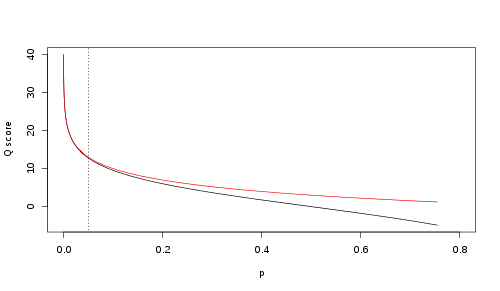
\includegraphics{./Probabilitymetrics.png}

}

\caption{\label{fig-Probabilitymetrics}Relationship between \emph{Q} and
\emph{p} using the Sanger (red) and Solexa (black) equations (described
above). The vertical dotted line indicates \(\mathbf{p}= 0.05\), or
equivalently, \(Q = 13\).}

\end{figure}

\hypertarget{encoding}{%
\subsubsection*{Encoding}\label{encoding}}
\addcontentsline{toc}{subsubsection}{Encoding}

The \emph{fastq} format had differente way of encoding the Phred quality
score along the time. Here a breif history of these changes is
presented.

\begin{itemize}
\tightlist
\item
  Sanger format can encode a Phred quality score from 0 to 93 using
  ASCII 33 to 126 (although in raw read data the Phred quality score
  rarely exceeds 60, higher scores are possible in assemblies or read
  maps).
\item
  Solexa/Illumina 1.0 format can encode a Solexa/Illumina quality score
  from -5 to 62 using ASCII 59 to 126 (although in raw read data Solexa
  scores from -5 to 40 only are expected)
\item
  Starting with Illumina 1.3 and before Illumina 1.8, the format encoded
  a Phred quality score from 0 to 62 using ASCII 64 to 126 (although in
  raw read data Phred scores from 0 to 40 only are expected).
\item
  Starting in Illumina 1.5 and before Illumina 1.8, the Phred scores 0
  to 2 have a slightly different meaning. The values 0 and 1 are no
  longer used and the value 2, encoded by ASCII 66 ``B''.
\end{itemize}

\begin{quote}
Sequencing Control Software, Version 2.6, (Catalog \# SY-960-2601, Part
\# 15009921 Rev.~A, November 2009, page 30) states the following:
\emph{If a read ends with a segment of mostly low quality (Q15 or
below), then all of the quality values in the segment are replaced with
a value of 2 (encoded as the letter B in Illumina's text-based encoding
of quality scores)\ldots{} This Q2 indicator does not predict a specific
error rate, but rather indicates that a specific final portion of the
read should not be used in further analyses.} Also, the quality score
encoded as ``B'' letter may occur internally within reads at least as
late as pipeline version 1.6, as shown in the following example:
\end{quote}

\begin{verbatim}
@HWI-EAS209_0006_FC706VJ:5:58:5894:21141#ATCACG/1
TTAATTGGTAAATAAATCTCCTAATAGCTTAGATNTTACCTTNNNNNNNNNNTAGTTTCTTGAGA
TTTGTTGGGGGAGACATTTTTGTGATTGCCTTGAT
+HWI-EAS209_0006_FC706VJ:5:58:5894:21141#ATCACG/1
efcfffffcfeefffcffffffddf`feed]`]_Ba_^__[YBBBBBBBBBBRTT\]][ dddd`
ddd^dddadd^BBBBBBBBBBBBBBBBBBBBBBBB
\end{verbatim}

An alternative interpretation of this ASCII encoding has been proposed.
Also, in Illumina runs using PhiX controls, the character `B' was
observed to represent an ``unknown quality score''. The error rate of
`B' reads was roughly 3 phred scores lower the mean observed score of a
given run.

\begin{itemize}
\tightlist
\item
  Starting in Illumina 1.8, the quality scores have basically returned
  to the use of the Sanger format (Phred+33).
\end{itemize}

OBItools follows the Sanger format. Nevertheless, It is possible to read
files encoded following the Solexa/Illumina format by applying a shift
of 62 (see the option \textbf{-\/-solexa} of the OBITools commands).

\hypertarget{file-extension}{%
\section{File extension}\label{file-extension}}

There is no standard file extension for a FASTQ file, but .fq and
.fastq, are commonly used.

\hypertarget{obitools-v4-tutorial}{%
\chapter{OBITools V4 Tutorial}\label{obitools-v4-tutorial}}

Here is a short tutorial on how to analyze DNA metabarcoding data
produced on Illumina sequencers using:

\begin{itemize}
\tightlist
\item
  the OBITools
\item
  some basic Unix commands
\end{itemize}

\hypertarget{wolves-diet-based-on-dna-metabarcoding}{%
\section{Wolves' diet based on DNA
metabarcoding}\label{wolves-diet-based-on-dna-metabarcoding}}

The data used in this tutorial correspond to the analysis of four wolf
scats, using the protocol published in Shehzad et al. (2012) for
assessing carnivore diet. After extracting DNA from the faeces, the DNA
amplifications were carried out using the primers
\texttt{TTAGATACCCCACTATGC} and \texttt{TAGAACAGGCTCCTCTAG} amplifiying
the \emph{12S-V5} region (Riaz et al. 2011), together with a wolf
blocking oligonucleotide.

The complete data set can be downloaded here: \href{wolf_diet.tgz}{the
tutorial dataset}

Once the data file is downloaded, using a UNIX terminal unarchive the
data from the \texttt{tgz} file.

\begin{Shaded}
\begin{Highlighting}[]
\FunctionTok{tar}\NormalTok{ zxvf wolf\_diet.tgz}
\end{Highlighting}
\end{Shaded}

That command create a new directory named \texttt{wolf\_data} containing
every required data files:

\begin{itemize}
\item
  \texttt{fastq\ \textless{}fastq\textgreater{}} files resulting of aGA
  IIx (Illumina) paired-end (2 x 108 bp) sequencing assay of DNA
  extracted and amplified from four wolf faeces:

  \begin{itemize}
  \tightlist
  \item
    \texttt{wolf\_F.fastq}
  \item
    \texttt{wolf\_R.fastq}
  \end{itemize}
\item
  the file describing the primers and tags used for all samples
  sequenced:

  \begin{itemize}
  \tightlist
  \item
    \texttt{wolf\_diet\_ngsfilter.txt} The tags correspond to short and
    specific sequences added on the 5\textquotesingle{} end of each
    primer to distinguish the different samples
  \end{itemize}
\item
  the file containing the reference database in a fasta format:

  \begin{itemize}
  \tightlist
  \item
    \texttt{db\_v05\_r117.fasta} This reference database has been
    extracted from the release 117 of EMBL using \texttt{obipcr}
  \end{itemize}
\end{itemize}

To not mix raw data and processed data a new directory called
\texttt{results} is created.

\begin{Shaded}
\begin{Highlighting}[]
\FunctionTok{mkdir}\NormalTok{ results}
\end{Highlighting}
\end{Shaded}

\hypertarget{step-by-step-analysis}{%
\section{Step by step analysis}\label{step-by-step-analysis}}

\hypertarget{recover-full-sequence-reads-from-forward-and-reverse-partial-reads}{%
\subsection{Recover full sequence reads from forward and reverse partial
reads}\label{recover-full-sequence-reads-from-forward-and-reverse-partial-reads}}

When using the result of a paired-end sequencing assay with supposedly
overlapping forward and reverse reads, the first step is to recover the
assembled sequence.

The forward and reverse reads of the same fragment are \emph{at the same
line position} in the two fastq files obtained after sequencing. Based
on these two files, the assembly of the forward and reverse reads is
done with the \texttt{obipairing} utility that aligns the two reads and
returns the reconstructed sequence.

In our case, the command is:

\begin{Shaded}
\begin{Highlighting}[]
\ExtensionTok{obipairing} \AttributeTok{{-}{-}min{-}identity}\OperatorTok{=}\NormalTok{0.8 }\DataTypeTok{\textbackslash{}}
           \AttributeTok{{-}{-}min{-}overlap}\OperatorTok{=}\NormalTok{10 }\DataTypeTok{\textbackslash{}}
           \AttributeTok{{-}F}\NormalTok{ wolf\_data/wolf\_F.fastq }\DataTypeTok{\textbackslash{}}
           \AttributeTok{{-}R}\NormalTok{ wolf\_data/wolf\_R.fastq }\DataTypeTok{\textbackslash{}}
           \OperatorTok{\textgreater{}}\NormalTok{ results/wolf.fastq }
\end{Highlighting}
\end{Shaded}

The \texttt{-\/-min-identity} and \texttt{-\/-min-overlap} options allow
discarding sequences with low alignment quality. If after the aligment,
the overlaping parts of the reads is shorter than 10 base pairs or the
similarity over this aligned region is below 80\% of identity, in the
output file, the forward and reverse reads are not aligned but
concatenated, and the value of the \texttt{mode} attribute in the
sequence header is set to \texttt{joined} instead of \texttt{alignment}.

\hypertarget{remove-unaligned-sequence-records}{%
\subsection{Remove unaligned sequence
records}\label{remove-unaligned-sequence-records}}

Unaligned sequences (:py\texttt{mode=joined}) cannot be used. The
following command allows removing them from the dataset:

\begin{Shaded}
\begin{Highlighting}[]
\ExtensionTok{obigrep} \AttributeTok{{-}p} \StringTok{\textquotesingle{}annotations.mode != "join"\textquotesingle{}} \DataTypeTok{\textbackslash{}}
\NormalTok{        results/wolf.fastq }\OperatorTok{\textgreater{}}\NormalTok{ results/wolf.ali.fastq}
\end{Highlighting}
\end{Shaded}

The \texttt{-p} requires a go like expression.
\texttt{annotations.mode\ !=\ "join"} means that if the value of the
\texttt{mode} annotation of a sequence is different from \texttt{join},
the corresponding sequence record will be kept.

The first sequence record of \texttt{wolf.ali.fastq} can be obtained
using the following command line:

\begin{Shaded}
\begin{Highlighting}[]
\FunctionTok{head} \AttributeTok{{-}n}\NormalTok{ 4 results/wolf.ali.fastq}
\end{Highlighting}
\end{Shaded}

The folling piece of code appears on thew window of tour terminal.

\begin{verbatim}
@HELIUM_000100422_612GNAAXX:7:108:5640:3823#0/1 {"ali_dir":"left","ali_length":62,"mode":"alignment","pairing_mismatches":{"(T:26)->(G:13)":62,"(T:34)->(G:18)":48},"score":484,"score_norm":0.968,"seq_a_single":46,"seq_ab_match":60,"seq_b_single":46}
ccgcctcctttagataccccactatgcttagccctaaacacaagtaattaatataacaaaattgttcgccagagtactaccggcaatagcttaaaactcaaaggacttggcggtgctttatacccttctagaggagcctgttctaaggaggcgg
+
CCCCCCCBCCCCCCCCCCCCCCCCCCCCCCBCCCCCBCCCCCCC<CcCccbe[`F`accXV<TA\RYU\\ee_e[XZ[XEEEEEEEEEE?EEEEEEEEEEDEEEEEEECCCCCCCCCCCCCCCCCCCCCCCACCCCCACCCCCCCCCCCCCCCC
\end{verbatim}

\hypertarget{assign-each-sequence-record-to-the-corresponding-samplemarker-combination}{%
\subsection{Assign each sequence record to the corresponding
sample/marker
combination}\label{assign-each-sequence-record-to-the-corresponding-samplemarker-combination}}

Each sequence record is assigned to its corresponding sample and marker
using the data provided in a text file (here
\texttt{wolf\_diet\_ngsfilter.txt}). This text file contains one line
per sample, with the name of the experiment (several experiments can be
included in the same file), the name of the tags (for example:
\texttt{aattaac} if the same tag has been used on each extremity of the
PCR products, or \texttt{aattaac:gaagtag} if the tags were different),
the sequence of the forward primer, the sequence of the reverse primer,
the letter \texttt{T} or \texttt{F} for sample identification using the
forward primer and tag only or using both primers and both tags,
respectively (see \texttt{obimultiplex} for details).

\begin{Shaded}
\begin{Highlighting}[]
\ExtensionTok{obimultiplex} \AttributeTok{{-}t}\NormalTok{ wolf\_data/wolf\_diet\_ngsfilter.txt }\DataTypeTok{\textbackslash{}}
             \AttributeTok{{-}u}\NormalTok{ results/unidentified.fastq }\DataTypeTok{\textbackslash{}}
\NormalTok{             results/wolf.ali.fastq }\DataTypeTok{\textbackslash{}}
             \OperatorTok{\textgreater{}}\NormalTok{ results/wolf.ali.assigned.fastq}
\end{Highlighting}
\end{Shaded}

This command creates two files:

\begin{itemize}
\tightlist
\item
  \texttt{unidentified.fastq} containing all the sequence records that
  were not assigned to a sample/marker combination
\item
  \texttt{wolf.ali.assigned.fastq} containing all the sequence records
  that were properly assigned to a sample/marker combination
\end{itemize}

Note that each sequence record of the \texttt{wolf.ali.assigned.fastq}
file contains only the barcode sequence as the sequences of primers and
tags are removed by the \texttt{obimultiplex} program. Information
concerning the experiment, sample, primers and tags is added as
attributes in the sequence header.

For instance, the first sequence record of
\texttt{wolf.ali.assigned.fastq} is:

\begin{verbatim}
@HELIUM_000100422_612GNAAXX:7:108:5640:3823#0/1_sub[28..127] {"ali_dir":"left","ali_length":62,"direction":"direct","experiment":"wolf_diet","forward_match":"ttagataccccactatgc","forward_mismatches":0,"forward_primer":"ttagataccccactatgc","forward_tag":"gcctcct","mode":"alignment","pairing_mismatches":{"(T:26)->(G:13)":35,"(T:34)->(G:18)":21},"reverse_match":"tagaacaggctcctctag","reverse_mismatches":0,"reverse_primer":"tagaacaggctcctctag","reverse_tag":"gcctcct","sample":"29a_F260619","score":484,"score_norm":0.968,"seq_a_single":46,"seq_ab_match":60,"seq_b_single":46}
ttagccctaaacacaagtaattaatataacaaaattgttcgccagagtactaccggcaatagcttaaaactcaaaggacttggcggtgctttataccctt
+
CCCBCCCCCBCCCCCCC<CcCccbe[`F`accXV<TA\RYU\\ee_e[XZ[XEEEEEEEEEE?EEEEEEEEEEDEEEEEEECCCCCCCCCCCCCCCCCCC
\end{verbatim}

\hypertarget{dereplicate-reads-into-uniq-sequences}{%
\subsection{Dereplicate reads into uniq
sequences}\label{dereplicate-reads-into-uniq-sequences}}

The same DNA molecule can be sequenced several times. In order to reduce
both file size and computations time, and to get easier interpretable
results, it is convenient to work with unique \emph{sequences} instead
of \emph{reads}. To \emph{dereplicate} such \emph{reads} into unique
\emph{sequences}, we use the \texttt{obiuniq} command.

\begin{longtable}[]{@{}
  >{\raggedright\arraybackslash}p{(\columnwidth - 0\tabcolsep) * \real{0.8611}}@{}}
\toprule()
\endhead
Definition: Dereplicate reads into unique sequences \\
\begin{minipage}[t]{\linewidth}\raggedright
\begin{enumerate}
\def\labelenumi{\arabic{enumi}.}
\tightlist
\item
  compare all the reads in a data set to each other
\item
  group strictly identical reads together
\item
  output the sequence for each group and its count in the original
  dataset (in this way, all duplicated reads are removed)
\end{enumerate}

Definition adapted from Seguritan and Rohwer (2001)
\end{minipage} \\
\bottomrule()
\end{longtable}

For dereplication, we use the \texttt{obiuniq} command with the
\texttt{-m\ sample}. The \texttt{-m\ sample} option is used to keep the
information of the samples of origin for each uniquesequence.

\begin{Shaded}
\begin{Highlighting}[]
\ExtensionTok{obiuniq} \AttributeTok{{-}m}\NormalTok{ sample }\DataTypeTok{\textbackslash{}}
\NormalTok{        results/wolf.ali.assigned.fastq }\DataTypeTok{\textbackslash{}}
        \OperatorTok{\textgreater{}}\NormalTok{ results/wolf.ali.assigned.uniq.fasta}
\end{Highlighting}
\end{Shaded}

Note that \texttt{obiuniq} returns a fasta file.

The first sequence record of \texttt{wolf.ali.assigned.uniq.fasta} is:

\begin{verbatim}
>HELIUM_000100422_612GNAAXX:7:93:6991:1942#0/1_sub[28..126] {"ali_dir":"left","ali_length":63,"count":1,"direction":"reverse","experiment":"wolf_diet","forward_match":"ttagataccccactatgc","forward_mismatches":0,"forward_primer":"ttagataccccactatgc","forward_tag":"gaatatc","merged_sample":{"26a_F040644":1},"mode":"alignment","pairing_mismatches":{"(A:10)->(G:34)":76,"(C:06)->(A:34)":58},"reverse_match":"tagaacaggctcctctag","reverse_mismatches":0,"reverse_primer":"tagaacaggctcctctag","reverse_tag":"gaatatc","score":730,"score_norm":0.968,"seq_a_single":45,"seq_ab_match":61,"seq_b_single":45}
ttagccctaaacataaacattcaataaacaagaatgttcgccagagaactactagcaaca
gcctgaaactcaaaggacttggcggtgctttatatccct
\end{verbatim}

The run of \texttt{obiuniq} has added two key=values entries in the
header of the fasta sequence:

\begin{itemize}
\tightlist
\item
  \texttt{"merged\_sample":\{"29a\_F260619":1\}}: this sequence have
  been found once in a single sample called \textbf{29a\_F260619}
\item
  \texttt{"count":1} : the total count for this sequence is \(1\)
\end{itemize}

To keep only these two attributes, we can use the \texttt{obiannotate}
command:

\begin{Shaded}
\begin{Highlighting}[]
\ExtensionTok{obiannotate} \AttributeTok{{-}k}\NormalTok{ count }\AttributeTok{{-}k}\NormalTok{ merged\_sample }\DataTypeTok{\textbackslash{}}
\NormalTok{  results/wolf.ali.assigned.uniq.fasta }\DataTypeTok{\textbackslash{}}
  \OperatorTok{\textgreater{}}\NormalTok{ results/wolf.ali.assigned.simple.fasta}
\end{Highlighting}
\end{Shaded}

The first five sequence records of
\texttt{wolf.ali.assigned.simple.fasta} become:

\begin{verbatim}
>HELIUM_000100422_612GNAAXX:7:26:18930:11105#0/1_sub[28..127] {"count":1,"merged_sample":{"29a_F260619":1}}
ttagccctaaacacaagtaattaatataacaaaatwattcgcyagagtactacmggcaat
agctyaaarctcamagrwcttggcggtgctttataccctt
>HELIUM_000100422_612GNAAXX:7:58:5711:11399#0/1_sub[28..127] {"count":1,"merged_sample":{"29a_F260619":1}}
ttagccctaaacacaagtaattaatataacaaaattattcgccagagtwctaccgssaat
agcttaaaactcaaaggactgggcggtgctttataccctt
>HELIUM_000100422_612GNAAXX:7:100:15836:9304#0/1_sub[28..127] {"count":1,"merged_sample":{"29a_F260619":1}}
ttagccctaaacatagataattacacaaacaaaattgttcaccagagtactagcggcaac
agcttaaaactcaaaggacttggcggtgctttataccctt
>HELIUM_000100422_612GNAAXX:7:55:13242:9085#0/1_sub[28..126] {"count":4,"merged_sample":{"26a_F040644":4}}
ttagccctaaacataaacattcaataaacaagagtgttcgccagagtactactagcaaca
gcctgaaactcaaaggacttggcggtgctttacatccct
>HELIUM_000100422_612GNAAXX:7:86:8429:13723#0/1_sub[28..127] {"count":7,"merged_sample":{"15a_F730814":5,"29a_F260619":2}}
ttagccctaaacacaagtaattaatataacaaaattattcgccagagtactaccggcaat
agcttaaaactcaaaggactcggcggtgctttataccctt
\end{verbatim}

\hypertarget{denoise-the-sequence-dataset}{%
\subsection{Denoise the sequence
dataset}\label{denoise-the-sequence-dataset}}

To have a set of sequences assigned to their corresponding samples does
not mean that all sequences are \emph{biologically} meaningful i.e.~some
of these sequences can contains PCR and/or sequencing errors, or
chimeras.

\hypertarget{tag-the-sequences-for-pcr-errors-sequence-variants}{%
\subsubsection*{Tag the sequences for PCR errors (sequence
variants)}\label{tag-the-sequences-for-pcr-errors-sequence-variants}}
\addcontentsline{toc}{subsubsection}{Tag the sequences for PCR errors
(sequence variants)}

The \texttt{obiclean} program tags sequence variants as potential error
generated during PCR amplification. We ask it to keep the {head}
sequences (\texttt{-H} option) that are sequences which are not variants
of another sequence with a count greater than 5\% of their own count
(\texttt{-r\ 0.05} option).

\begin{Shaded}
\begin{Highlighting}[]
\ExtensionTok{obiclean} \AttributeTok{{-}s}\NormalTok{ sample }\AttributeTok{{-}r}\NormalTok{ 0.05 }\AttributeTok{{-}H} \DataTypeTok{\textbackslash{}}
\NormalTok{  results/wolf.ali.assigned.simple.fasta }\DataTypeTok{\textbackslash{}}
      \OperatorTok{\textgreater{}}\NormalTok{ results/wolf.ali.assigned.simple.clean.fasta }
\end{Highlighting}
\end{Shaded}

One of the sequence records of
\texttt{wolf.ali.assigned.simple.clean.fasta} is:

\begin{verbatim}
>HELIUM_000100422_612GNAAXX:7:66:4039:8016#0/1_sub[28..127] {"count":17,"merged_sample":{"13a_F730603":17},"obiclean_head":true,"obiclean_headcount":1,"obiclean_internalcount":0,"obi
clean_samplecount":1,"obiclean_singletoncount":0,"obiclean_status":{"13a_F730603":"h"},"obiclean_weight":{"13a_F730603":25}}
ctagccttaaacacaaatagttatgcaaacaaaactattcgccagagtactaccggcaac
agcccaaaactcaaaggacttggcggtgcttcacaccctt
\end{verbatim}

To remove such sequences as much as possible, we first discard rare
sequences and then rsequence variants that likely correspond to
artifacts.

\hypertarget{get-some-statistics-about-sequence-counts}{%
\subsubsection*{Get some statistics about sequence
counts}\label{get-some-statistics-about-sequence-counts}}
\addcontentsline{toc}{subsubsection}{Get some statistics about sequence
counts}

\begin{Shaded}
\begin{Highlighting}[]
\ExtensionTok{obicount}\NormalTok{ results/wolf.ali.assigned.simple.clean.fasta}
\end{Highlighting}
\end{Shaded}

\begin{verbatim}
time="2023-02-23T18:43:37+01:00" level=info msg="Appending results/wolf.ali.assigned.simple.clean.fasta file\n"
 2749 36409 273387
\end{verbatim}

The dataset contains \(4313\) sequences variant corresponding to 42452
sequence reads. Most of the variants occur only a single time in the
complete dataset and are usualy named \emph{singletons}

\begin{Shaded}
\begin{Highlighting}[]
\ExtensionTok{obigrep} \AttributeTok{{-}p} \StringTok{\textquotesingle{}sequence.Count() == 1\textquotesingle{}}\NormalTok{ results/wolf.ali.assigned.simple.clean.fasta }\DataTypeTok{\textbackslash{}}
    \KeywordTok{|} \ExtensionTok{obicount}
\end{Highlighting}
\end{Shaded}

\begin{verbatim}
time="2023-02-23T18:43:37+01:00" level=info msg="Reading sequences from stdin in guessed\n"
time="2023-02-23T18:43:37+01:00" level=info msg="Appending results/wolf.ali.assigned.simple.clean.fasta file\n"
time="2023-02-23T18:43:37+01:00" level=info msg="On output use JSON headers"
 2623 2623 261217
\end{verbatim}

In that dataset sigletons corresponds to \(3511\) variants.

Using \emph{R} and the \texttt{ROBIFastread} package able to read
headers of the fasta files produced by \emph{OBITools}, we can get more
complete statistics on the distribution of occurrencies.

\begin{Shaded}
\begin{Highlighting}[]
\FunctionTok{library}\NormalTok{(ROBIFastread)}
\FunctionTok{library}\NormalTok{(ggplot2)}

\NormalTok{seqs }\OtherTok{\textless{}{-}} \FunctionTok{read\_obifasta}\NormalTok{(}\StringTok{"results/wolf.ali.assigned.simple.clean.fasta"}\NormalTok{,}\AttributeTok{keys=}\StringTok{"count"}\NormalTok{)}

\FunctionTok{ggplot}\NormalTok{(}\AttributeTok{data =}\NormalTok{ seqs,  }\AttributeTok{mapping=}\FunctionTok{aes}\NormalTok{(}\AttributeTok{x =}\NormalTok{ count)) }\SpecialCharTok{+}
  \FunctionTok{geom\_histogram}\NormalTok{(}\AttributeTok{bins=}\DecValTok{100}\NormalTok{) }\SpecialCharTok{+}
  \FunctionTok{scale\_y\_sqrt}\NormalTok{() }\SpecialCharTok{+}
  \FunctionTok{scale\_x\_sqrt}\NormalTok{() }\SpecialCharTok{+}
  \FunctionTok{geom\_vline}\NormalTok{(}\AttributeTok{xintercept =} \DecValTok{10}\NormalTok{, }\AttributeTok{col=}\StringTok{"red"}\NormalTok{, }\AttributeTok{lty=}\DecValTok{2}\NormalTok{) }\SpecialCharTok{+}
  \FunctionTok{xlab}\NormalTok{(}\StringTok{"number of occurrencies of a variant"}\NormalTok{) }
\end{Highlighting}
\end{Shaded}

\begin{figure}[H]

{\centering 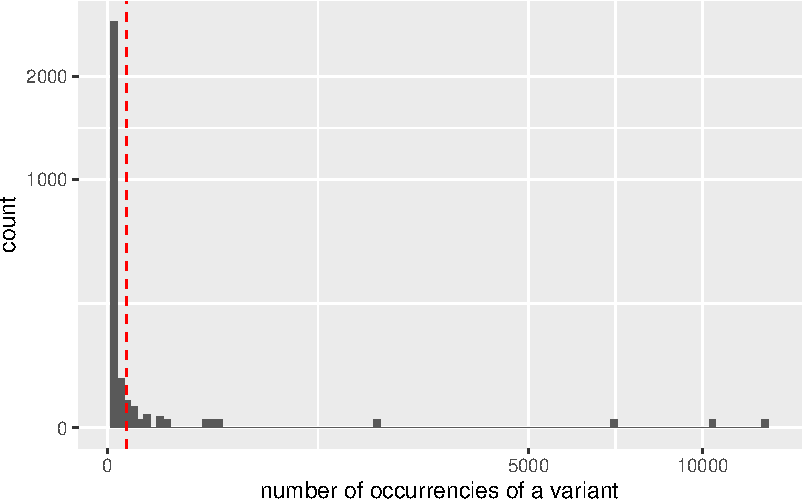
\includegraphics{./tutorial_files/figure-pdf/unnamed-chunk-9-1.pdf}

}

\end{figure}

In a similar way it is also possible to plot the distribution of the
sequence length.

\begin{Shaded}
\begin{Highlighting}[]
\FunctionTok{ggplot}\NormalTok{(}\AttributeTok{data =}\NormalTok{ seqs,  }\AttributeTok{mapping=}\FunctionTok{aes}\NormalTok{(}\AttributeTok{x =} \FunctionTok{nchar}\NormalTok{(sequence))) }\SpecialCharTok{+}
  \FunctionTok{geom\_histogram}\NormalTok{() }\SpecialCharTok{+}
  \FunctionTok{scale\_y\_log10}\NormalTok{() }\SpecialCharTok{+}
  \FunctionTok{geom\_vline}\NormalTok{(}\AttributeTok{xintercept =} \DecValTok{80}\NormalTok{, }\AttributeTok{col=}\StringTok{"red"}\NormalTok{, }\AttributeTok{lty=}\DecValTok{2}\NormalTok{) }\SpecialCharTok{+}
  \FunctionTok{xlab}\NormalTok{(}\StringTok{"sequence lengths in base pair"}\NormalTok{)}
\end{Highlighting}
\end{Shaded}

\begin{figure}[H]

{\centering 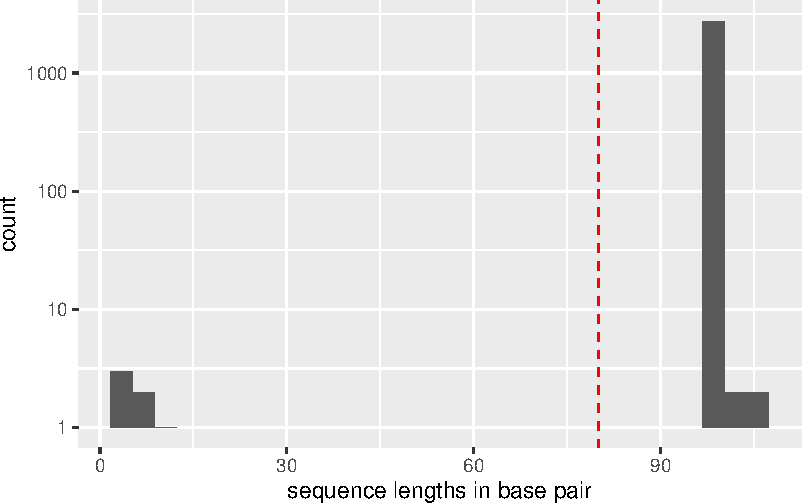
\includegraphics{./tutorial_files/figure-pdf/unnamed-chunk-10-1.pdf}

}

\end{figure}

\hypertarget{keep-only-the-sequences-having-a-count-greater-or-equal-to-10-and-a-length-shorter-than-80-bp}{%
\subsubsection*{Keep only the sequences having a count greater or equal
to 10 and a length shorter than 80
bp}\label{keep-only-the-sequences-having-a-count-greater-or-equal-to-10-and-a-length-shorter-than-80-bp}}
\addcontentsline{toc}{subsubsection}{Keep only the sequences having a
count greater or equal to 10 and a length shorter than 80 bp}

Based on the previous observation, we set the cut-off for keeping
sequences for further analysis to a count of 10. To do this, we use the
\texttt{obigrep\ \textless{}scripts/obigrep\textgreater{}} command. The
\texttt{-p\ \textquotesingle{}count\textgreater{}=10\textquotesingle{}}
option means that the \texttt{python} expression
:py\texttt{count\textgreater{}=10} must be evaluated to :py\texttt{True}
for each sequence to be kept. Based on previous knowledge we also remove
sequences with a length shorter than 80 bp (option -l) as we know that
the amplified 12S-V5 barcode for vertebrates must have a length around
100bp.

\begin{Shaded}
\begin{Highlighting}[]
\ExtensionTok{obigrep} \AttributeTok{{-}l}\NormalTok{ 80 }\AttributeTok{{-}p} \StringTok{\textquotesingle{}sequence.Count() \textgreater{}= 10\textquotesingle{}}\NormalTok{ results/wolf.ali.assigned.simple.clean.fasta }\DataTypeTok{\textbackslash{}}
    \OperatorTok{\textgreater{}}\NormalTok{ results/wolf.ali.assigned.simple.clean.c10.l80.fasta}
\end{Highlighting}
\end{Shaded}

The first sequence record of
\texttt{results/wolf.ali.assigned.simple.clean.c10.l80.fasta} is:

\begin{verbatim}
>HELIUM_000100422_612GNAAXX:7:22:2603:18023#0/1_sub[28..127] {"count":12182,"merged_sample":{"15a_F730814":7559,"29a_F260619":4623},"obiclean_head":true,"obiclean_headcount":2,"obiclean_internalcount":0,"obiclean_samplecount":2,"obiclean_singletoncount":0,"obiclean_status":{"15a_F730814":"h","29a_F260619":"h"},"obiclean_weight":{"15a_F730814":9165,"29a_F260619":6275}}
ttagccctaaacacaagtaattaatataacaaaattattcgccagagtactaccggcaat
agcttaaaactcaaaggacttggcggtgctttataccctt
\end{verbatim}

At that time in the data cleanning we have conserved :

\begin{Shaded}
\begin{Highlighting}[]
\ExtensionTok{obicount}\NormalTok{ results/wolf.ali.assigned.simple.clean.c10.l80.fasta}
\end{Highlighting}
\end{Shaded}

\begin{verbatim}
time="2023-02-23T18:43:40+01:00" level=info msg="Appending results/wolf.ali.assigned.simple.clean.c10.l80.fasta file\n"
 26 31337 2585
\end{verbatim}

\hypertarget{taxonomic-assignment-of-sequences}{%
\subsection{Taxonomic assignment of
sequences}\label{taxonomic-assignment-of-sequences}}

Once denoising has been done, the next step in diet analysis is to
assign the barcodes to the corresponding species in order to get the
complete list of species associated to each sample.

Taxonomic assignment of sequences requires a reference database
compiling all possible species to be identified in the sample.
Assignment is then done based on sequence comparison between sample
sequences and reference sequences.

\hypertarget{download-the-taxonomy}{%
\subsubsection*{Download the taxonomy}\label{download-the-taxonomy}}
\addcontentsline{toc}{subsubsection}{Download the taxonomy}

It is always possible to download the complete taxonomy from NCBI using
the following commands.

\begin{Shaded}
\begin{Highlighting}[]
\FunctionTok{mkdir}\NormalTok{ TAXO}
\BuiltInTok{cd}\NormalTok{ TAXO}
\ExtensionTok{curl}\NormalTok{ http://ftp.ncbi.nih.gov/pub/taxonomy/taxdump.tar.gz }\DataTypeTok{\textbackslash{}}
   \KeywordTok{|} \FunctionTok{tar} \AttributeTok{{-}zxvf} \AttributeTok{{-}}
\BuiltInTok{cd}\NormalTok{ ..}
\end{Highlighting}
\end{Shaded}

For people have a low speed internet connection, a copy of the
\texttt{taxdump.tar.gz} file is provided in the wolf\_data directory.
The NCBI taxonomy is dayly updated, but the one provided here is ok for
running this tutorial.

To build the TAXO directory from the provided \texttt{taxdump.tar.gz},
you need to execute the following commands

\begin{Shaded}
\begin{Highlighting}[]
\FunctionTok{mkdir}\NormalTok{ TAXO}
\BuiltInTok{cd}\NormalTok{ TAXO}
\FunctionTok{tar}\NormalTok{ zxvf wolf\_data/taxdump.tar.gz }
\BuiltInTok{cd}\NormalTok{ ..}
\end{Highlighting}
\end{Shaded}

\hypertarget{build-a-reference-database}{%
\subsubsection*{Build a reference
database}\label{build-a-reference-database}}
\addcontentsline{toc}{subsubsection}{Build a reference database}

One way to build the reference database is to use the \texttt{obipcr}
program to simulate a PCR and extract all sequences from a general
purpose DNA database such as genbank or EMBL that can be amplified
\emph{in silico} by the two primers (here \textbf{TTAGATACCCCACTATGC}
and \textbf{TAGAACAGGCTCCTCTAG}) used for PCR amplification.

The two steps to build this reference database would then be

\begin{enumerate}
\def\labelenumi{\arabic{enumi}.}
\item
  Today, the easiest database to download is \emph{Genbank}. But this
  will take you more than a day and occupy more than half a terabyte on
  your hard drive. In the \texttt{wolf\_data} directory, a shell script
  called \texttt{download\_gb.sh} is provided to perform this task. It
  requires that the programs \texttt{wget2} and \texttt{curl} are
  available on your computer.
\item
  Use \texttt{obipcr} to simulate amplification and build a reference
  database based on the putatively amplified barcodes and their recorded
  taxonomic information.
\end{enumerate}

As these steps can take a long time (about a day for the download and an
hour for the PCR), we already provide the reference database produced by
the following commands so you can skip its construction. Note that as
the Genbank and taxonomic database evolve frequently, if you run the
following commands you may get different results.

\hypertarget{download-the-sequences}{%
\paragraph*{Download the sequences}\label{download-the-sequences}}
\addcontentsline{toc}{paragraph}{Download the sequences}

\begin{Shaded}
\begin{Highlighting}[]
\FunctionTok{mkdir}\NormalTok{ genbank}
\BuiltInTok{cd}\NormalTok{ genbank}
\ExtensionTok{../wolf\_data/install\_gb.sh}
\BuiltInTok{cd}\NormalTok{ ..}
\end{Highlighting}
\end{Shaded}

DO NOT RUN THIS COMMAND EXCEPT IF YOU ARE REALLY CONSIENT OF THE TIME
AND DISK SPACE REQUIRED.

\hypertarget{use-obipcr-to-simulate-an-in-silico-pcr}{%
\paragraph*{Use obipcr to simulate an in silico`
PCR}\label{use-obipcr-to-simulate-an-in-silico-pcr}}
\addcontentsline{toc}{paragraph}{Use obipcr to simulate an in silico`
PCR}

\begin{Shaded}
\begin{Highlighting}[]
\ExtensionTok{obipcr} \AttributeTok{{-}t}\NormalTok{ TAXO }\AttributeTok{{-}e}\NormalTok{ 3 }\AttributeTok{{-}l}\NormalTok{ 50 }\AttributeTok{{-}L}\NormalTok{ 150 }\DataTypeTok{\textbackslash{} }
       \ExtensionTok{{-}{-}forward}\NormalTok{ TTAGATACCCCACTATGC }\DataTypeTok{\textbackslash{}}
       \AttributeTok{{-}{-}reverse}\NormalTok{ TAGAACAGGCTCCTCTAG }\DataTypeTok{\textbackslash{}}
       \AttributeTok{{-}{-}no{-}order} \DataTypeTok{\textbackslash{}}
\NormalTok{       genbank/Release{-}251/gb}\PreprocessorTok{*}\NormalTok{.seq.gz}
       \OperatorTok{\textgreater{}}\NormalTok{ results/v05.pcr.fasta}
\end{Highlighting}
\end{Shaded}

Note that the primers must be in the same order both in
\texttt{wolf\_diet\_ngsfilter.txt} and in the \texttt{obipcr} command.
The part of the path indicating the \emph{Genbank} release can change.
Please check in your genbank directory the exact name of your release.

\hypertarget{clean-the-database}{%
\paragraph*{Clean the database}\label{clean-the-database}}
\addcontentsline{toc}{paragraph}{Clean the database}

\begin{enumerate}
\def\labelenumi{\arabic{enumi}.}
\tightlist
\item
  filter sequences so that they have a good taxonomic description at the
  species, genus, and family levels (\texttt{obigrep} command command
  below).
\item
  remove redundant sequences (\texttt{obiuniq} command below).
\item
  ensure that the dereplicated sequences have a taxid at the family
  level (\texttt{obigrep} command below).
\item
  ensure that sequences each have a unique identification
  (\texttt{obiannotate} command below)
\end{enumerate}

\begin{Shaded}
\begin{Highlighting}[]
\ExtensionTok{obigrep} \AttributeTok{{-}t}\NormalTok{ TAXO }\DataTypeTok{\textbackslash{}}
          \AttributeTok{{-}{-}require{-}rank}\NormalTok{ species }\DataTypeTok{\textbackslash{}}
          \AttributeTok{{-}{-}require{-}rank}\NormalTok{ genus }\DataTypeTok{\textbackslash{}}
          \AttributeTok{{-}{-}require{-}rank}\NormalTok{ family }\DataTypeTok{\textbackslash{}}
\NormalTok{          results/v05.ecopcr }\OperatorTok{\textgreater{}}\NormalTok{ results/v05\_clean.fasta}

\ExtensionTok{obiuniq} \AttributeTok{{-}c}\NormalTok{ taxid }\DataTypeTok{\textbackslash{}}
\NormalTok{        results/v05\_clean.fasta }\DataTypeTok{\textbackslash{}}
        \OperatorTok{\textgreater{}}\NormalTok{ results/v05\_clean\_uniq.fasta}

\ExtensionTok{obirefidx} \AttributeTok{{-}t}\NormalTok{ TAXO results/v05\_clean\_uniq.fasta }\DataTypeTok{\textbackslash{}}
        \OperatorTok{\textgreater{}}\NormalTok{ results/v05\_clean\_uniq.indexed.fasta}
\end{Highlighting}
\end{Shaded}

Warning

From now on, for the sake of clarity, the following commands will use
the filenames of the files provided with the tutorial. If you decided to
run the last steps and use the files you have produced,
you\textquotesingle ll have to use
\texttt{results/v05\_clean\_uniq.indexed.fasta} instead of
\texttt{wolf\_data/db\_v05\_r117.indexed.fasta}.

\hypertarget{assign-each-sequence-to-a-taxon}{%
\subsection{Assign each sequence to a
taxon}\label{assign-each-sequence-to-a-taxon}}

Once the reference database is built, taxonomic assignment can be
carried out using the \texttt{obitag} command.

\begin{Shaded}
\begin{Highlighting}[]
\ExtensionTok{obitag} \AttributeTok{{-}t}\NormalTok{ TAXO }\AttributeTok{{-}R}\NormalTok{ wolf\_data/db\_v05\_r117.indexed.fasta }\DataTypeTok{\textbackslash{}}
\NormalTok{       results/wolf.ali.assigned.simple.clean.c10.l80.fasta }\DataTypeTok{\textbackslash{}}
       \OperatorTok{\textgreater{}}\NormalTok{ results/wolf.ali.assigned.simple.clean.c10.l80.taxo.fasta}
\end{Highlighting}
\end{Shaded}

The \texttt{obitag} adds several attributes in the sequence record
header, among them:

\begin{itemize}
\tightlist
\item
  obitag\_bestmatch=ACCESSION where ACCESSION is the id of hte sequence
  in the reference database that best aligns to the query sequence;
\item
  obitag\_bestid=FLOAT where FLOAT*100 is the percentage of identity
  between the best match sequence and the query sequence;
\item
  taxid=TAXID where TAXID is the final assignation of the sequence by
  \texttt{obitag}
\item
  scientific\_name=NAME where NAME is the scientific name of the
  assigned taxid.
\end{itemize}

The first sequence record of
\texttt{wolf.ali.assigned.simple.clean.c10.l80.taxo.fasta} is:

\begin{Shaded}
\begin{Highlighting}[]
\OperatorTok{\textgreater{}}\NormalTok{HELIUM\_000100422\_612GNAAXX:7:81:18704:12346\#0/1\_sub[28..126] }\DataTypeTok{\{}\StringTok{"count"}\DataTypeTok{:88}\OperatorTok{,}\StringTok{"merged\_sample"}\DataTypeTok{:\{}\StringTok{"26a\_F040644"}\DataTypeTok{:88\}}\OperatorTok{,}\StringTok{"obiclean\_head"}\DataTypeTok{:true}\OperatorTok{,}\StringTok{"obiclean\_headcount"}\DataTypeTok{:1}\OperatorTok{,}\StringTok{"obiclean\_internalcount"}\DataTypeTok{:0}\OperatorTok{,}\StringTok{"obiclean\_samplecount"}\DataTypeTok{:1}\OperatorTok{,}\StringTok{"obiclean\_singletoncount"}\DataTypeTok{:0}\OperatorTok{,}\StringTok{"obiclean\_status"}\DataTypeTok{:\{}\StringTok{"26a\_F040644"}\DataTypeTok{:}\StringTok{"h"}\DataTypeTok{\}}\OperatorTok{,}\StringTok{"obiclean\_weight"}\DataTypeTok{:\{}\StringTok{"26a\_F040644"}\DataTypeTok{:208\}}\OperatorTok{,}\StringTok{"obitag\_bestid"}\DataTypeTok{:0.9207920792079208}\OperatorTok{,}\StringTok{"obitag\_bestmatch"}\DataTypeTok{:}\StringTok{"AY769263"}\OperatorTok{,}\StringTok{"obitag\_difference"}\DataTypeTok{:8}\OperatorTok{,}\StringTok{"obitag\_match\_count"}\DataTypeTok{:1}\OperatorTok{,}\StringTok{"obitag\_rank"}\DataTypeTok{:}\StringTok{"clade"}\OperatorTok{,}\StringTok{"scientific\_name"}\DataTypeTok{:}\StringTok{"Boreoeutheria"}\OperatorTok{,}\StringTok{"taxid"}\DataTypeTok{:1437010\}}
\ExtensionTok{ttagccctaaacataaacattcaataaacaagaatgttcgccagaggactactagcaata}
\ExtensionTok{gcttaaaactcaaaggacttggcggtgctttatatccct}
\end{Highlighting}
\end{Shaded}

\hypertarget{generate-the-final-result-table}{%
\subsection{Generate the final result
table}\label{generate-the-final-result-table}}

Some unuseful attributes can be removed at this stage.

\begin{itemize}
\tightlist
\item
  obiclean\_head
\item
  obiclean\_headcount
\item
  obiclean\_internalcount
\item
  obiclean\_samplecount
\item
  obiclean\_singletoncount
\end{itemize}

\begin{Shaded}
\begin{Highlighting}[]
\ExtensionTok{obiannotate}  \AttributeTok{{-}{-}delete{-}tag}\OperatorTok{=}\NormalTok{obiclean\_head }\DataTypeTok{\textbackslash{}}
             \AttributeTok{{-}{-}delete{-}tag}\OperatorTok{=}\NormalTok{obiclean\_headcount }\DataTypeTok{\textbackslash{}}
             \AttributeTok{{-}{-}delete{-}tag}\OperatorTok{=}\NormalTok{obiclean\_internalcount }\DataTypeTok{\textbackslash{}}
             \AttributeTok{{-}{-}delete{-}tag}\OperatorTok{=}\NormalTok{obiclean\_samplecount }\DataTypeTok{\textbackslash{}}
             \AttributeTok{{-}{-}delete{-}tag}\OperatorTok{=}\NormalTok{obiclean\_singletoncount }\DataTypeTok{\textbackslash{}}
\NormalTok{  results/wolf.ali.assigned.simple.clean.c10.l80.taxo.fasta }\DataTypeTok{\textbackslash{}}
  \OperatorTok{\textgreater{}}\NormalTok{ results/wolf.ali.assigned.simple.clean.c10.l80.taxo.ann.fasta}
\end{Highlighting}
\end{Shaded}

The first sequence record of
\texttt{wolf.ali.assigned.simple.c10.l80.clean.taxo.ann.fasta} is then:

\begin{verbatim}
>HELIUM_000100422_612GNAAXX:7:84:16335:5083#0/1_sub[28..126] {"count":96,"merged_sample":{"26a_F040644":11,"29a_F260619":85},"obiclean_status":{"26a_F040644":"s","29a_F260619":"h"},"obiclean_weight":{"26a_F040644":14,"29a_F260619":110},"obitag_bestid":0.9595959595959596,"obitag_bestmatch":"AC187326","obitag_difference":4,"obitag_match_count":1,"obitag_rank":"subspecies","scientific_name":"Canis lupus familiaris","taxid":9615}
ttagccctaaacataagctattccataacaaaataattcgccagagaactactagcaaca
gattaaacctcaaaggacttggcagtgctttatacccct
\end{verbatim}

\hypertarget{looking-at-the-data-in-r}{%
\subsection{Looking at the data in R}\label{looking-at-the-data-in-r}}

\begin{Shaded}
\begin{Highlighting}[]
\FunctionTok{library}\NormalTok{(ROBIFastread)}
\FunctionTok{library}\NormalTok{(vegan)}
\end{Highlighting}
\end{Shaded}

\begin{verbatim}
Le chargement a nécessité le package : permute
\end{verbatim}

\begin{verbatim}
Le chargement a nécessité le package : lattice
\end{verbatim}

\begin{verbatim}
This is vegan 2.6-4
\end{verbatim}

\begin{Shaded}
\begin{Highlighting}[]
\FunctionTok{library}\NormalTok{(magrittr)}
 

\NormalTok{diet\_data }\OtherTok{\textless{}{-}} \FunctionTok{read\_obifasta}\NormalTok{(}\StringTok{"results/wolf.ali.assigned.simple.clean.c10.l80.taxo.fasta"}\NormalTok{) }
\NormalTok{diet\_data }\SpecialCharTok{\%\textless{}\textgreater{}\%} \FunctionTok{extract\_features}\NormalTok{(}\StringTok{"obitag\_bestmatch"}\NormalTok{,}\StringTok{"obitag\_rank"}\NormalTok{,}\StringTok{"scientific\_name"}\NormalTok{,}\StringTok{\textquotesingle{}taxid\textquotesingle{}}\NormalTok{)}

\NormalTok{diet\_tab }\OtherTok{\textless{}{-}} \FunctionTok{extract\_readcount}\NormalTok{(diet\_data,}\AttributeTok{key=}\StringTok{"obiclean\_weight"}\NormalTok{)}
\NormalTok{diet\_tab}
\end{Highlighting}
\end{Shaded}

\begin{verbatim}
4 x 26 sparse Matrix of class "dgCMatrix"
\end{verbatim}

\begin{verbatim}
  [[ suppressing 26 column names 'HELIUM_000100422_612GNAAXX:7:100:4828:3492#0/1_sub[28..127]', 'HELIUM_000100422_612GNAAXX:7:7:2880:4021#0/1_sub[28..127]', 'HELIUM_000100422_612GNAAXX:7:7:18108:9040#0/1_sub[28..126]' ... ]]
\end{verbatim}

\begin{verbatim}
                                                                            
13a_F730603 22  . 9  19 25  1  .  .  .   .  .  .   .  .  . 20  .    .   .  .
29a_F260619  . 44 .   1  . 13  . 25  .   .  . 16 391  .  .  .  . 6275 110  .
15a_F730814  .  . 4   5  .  .  .  .  .   .  .  .   .  .  .  .  . 9138   .  .
26a_F040644  .  . . 481  .  . 14  . 43 208 72  .   . 52 88  . 31    .  14 18
                                   
13a_F730603     .  .  .   . 15 8409
29a_F260619     .  .  . 353  .    .
15a_F730814     .  .  .   .  .    .
26a_F040644 12265 15 17   .  .    .
\end{verbatim}

\begin{description}
\item[This file contains 26 sequences. You can deduce the diet of each
sample:]
\begin{itemize}
\tightlist
\item[]
\item
  13a\_F730603: Cervus elaphus
\item
  15a\_F730814: Capreolus capreolus
\item
  26a\_F040644: Marmota sp. (according to the location, it is Marmota
  marmota)
\item
  29a\_F260619: Capreolus capreolus
\end{itemize}
\end{description}

Note that we also obtained a few wolf sequences although a wolf-blocking
oligonucleotide was used.

\part{The \emph{OBITools V4} commands}

\hypertarget{specifying-the-data-input-to-obitools-commands}{%
\chapter{\texorpdfstring{Specifying the data input to \emph{OBITools}
commands}{Specifying the data input to OBITools commands}}\label{specifying-the-data-input-to-obitools-commands}}

\hypertarget{specifying-input-format}{%
\section{Specifying input format}\label{specifying-input-format}}

Five sequence formats are accepted for input files. \emph{Fasta}
(Section~\ref{sec-fasta}) and \emph{Fastq} (Section~\ref{sec-fastq}) are
the main ones, EMBL and Genbank allow the use of flat files produced by
these two international databases. The last one, ecoPCR, is maintained
for compatibility with previous \emph{OBITools} and allows to read
\emph{ecoPCR} outputs as sequence files.

\begin{itemize}
\tightlist
\item
  \texttt{-\/-ecopcr} : Read data following the \emph{ecoPCR} output
  format.
\item
  \texttt{-\/-embl} Read data following the \emph{EMBL} flatfile format.
\item
  \texttt{-\/-genbank} Read data following the \emph{Genbank} flatfile
  format.
\end{itemize}

Several encoding schemes have been proposed for quality scores in
\emph{Fastq} format. Currently, \emph{OBITools} considers Sanger
encoding as the standard. For reasons of compatibility with older
datasets produced with \emph{Solexa} sequencers, it is possible, by
using the following option, to force the use of the corresponding
quality encoding scheme when reading these older files.

\begin{itemize}
\tightlist
\item
  \texttt{-\/-solexa} Decodes quality string according to the Solexa
  specification. (default: false)
\end{itemize}

\hypertarget{controling-obitools-outputs}{%
\chapter{Controling OBITools
outputs}\label{controling-obitools-outputs}}

\hypertarget{specifying-output-format}{%
\section{Specifying output format}\label{specifying-output-format}}

Only two output sequence formats are supported by OBITools, Fasta and
Fastq. Fastq is used when output sequences are associated with quality
information. Otherwise, Fasta is the default format. However, it is
possible to force the output format by using one of the following two
options. Forcing the use of Fasta results in the loss of quality
information. Conversely, when the Fastq format is forced with sequences
that have no quality data, dummy qualities set to 40 for each nucleotide
are added.

\begin{itemize}
\tightlist
\item
  \texttt{-\/-fasta-output} Read data following the ecoPCR output
  format.
\item
  \texttt{-\/-fastq-output} Read data following the EMBL flatfile
  format.
\end{itemize}

OBITools allows multiple input files to be specified for a single
command.

\begin{itemize}
\tightlist
\item
  \texttt{-\/-no-order} When several input files are provided, indicates
  that there is no order among them. (default: false). Using such option
  can increase a lot the processing of the data.
\end{itemize}

\hypertarget{the-fasta-and-fastq-annotations-format}{%
\section{The Fasta and Fastq annotations
format}\label{the-fasta-and-fastq-annotations-format}}

OBITools extend the \protect\hyperlink{the-fasta-sequence-format}{Fasta}
and \protect\hyperlink{the-fastq-sequence-format}{Fastq} formats by
introducing a format for the title lines of these formats allowing to
annotate every sequence. While the previous version of OBITools used an
\emph{ad-hoc} format for these annotation, this new version introduce
the usage of the standard JSON format to store them.

On input, OBITools automatically recognize the format of the
annotations, but two options allows to force the parsing following one
of them. You should normally not need to use these options.

\begin{itemize}
\item
  \texttt{-\/-input-OBI-header} FASTA/FASTQ title line annotations
  follow OBI format. (default: false)
\item
  \texttt{-\/-input-json-header} FASTA/FASTQ title line annotations
  follow json format. (default: false)
\end{itemize}

On output, by default annotation are formatted using the new JSON
format. For compatibility with previous version of OBITools and with
external scripts and software, it is possible to force the usage of the
previous OBITools format.

\begin{itemize}
\item
  \texttt{-\/-output-OBI-header\textbar{}-O} output FASTA/FASTQ title
  line annotations follow OBI format. (default: false)
\item
  \texttt{-\/-output-json-header} output FASTA/FASTQ title line
  annotations follow json format. (default: false)
\end{itemize}

\hypertarget{options-common-to-most-of-the-obitools-commands}{%
\chapter{\texorpdfstring{Options common to most of the \emph{OBITools}
commands}{Options common to most of the OBITools commands}}\label{options-common-to-most-of-the-obitools-commands}}

\hypertarget{helpful-options}{%
\section{Helpful options}\label{helpful-options}}

\begin{description}
\item[\textbf{-\/-help}, \textbf{-h}]
Display a friendly help message.
\end{description}

\textbf{-\/-no-progressbar}

\hypertarget{system-related-options}{%
\section{System related options}\label{system-related-options}}

\textbf{Managing parallel execution of tasks}

A new feature of \emph{OBITools} V4 is the ability to run multiple tasks
in parallel, reading files, calculating on the data, formatting and
writing the results. Each of these tasks can itself be parallelized by
dividing the data into batches and running the calculation on several
batches in parallel. This allows the overall calculation time of an
\emph{OBITools} command to be reduced considerably. The parameters
organizing the parallel calculation are determined automatically to use
the maximum capacity of your computer. But in some circumstances, it is
necessary to override these default settings either to try to optimize
the computation on a given machine, or to limit the OBITools to using
only a part of the computational capacity. There are two options for
doing this.

\begin{description}
\item[\textbf{-\/-max-cpu}]
OBITools V4 are able to run in parallel on all the CPU cores available
on the computer. It is sometime required to limit the computation to a
smaller number of cores. That option specify the maximum number of cores
that the OBITools command can use. This behaviour can also be set up
using the \texttt{OBIMAXCPU} environment variable.
\end{description}

\textbf{-\/-workers}, \textbf{-w}

If your computer has 8 cores, but you want to limit \emph{OBITools} to
use only two of them you have several solution:

\begin{itemize}
\item
  If you want to set the limit for a single execution you can use the
  \textbf{--max-cpu} option

\begin{Shaded}
\begin{Highlighting}[]
\ExtensionTok{obiconvert} \AttributeTok{{-}{-}max{-}cpu}\NormalTok{ 2 }\AttributeTok{{-}{-}fasta{-}output}\NormalTok{ data.fastq }\OperatorTok{\textgreater{}}\NormalTok{ data.fasta}
\end{Highlighting}
\end{Shaded}

  or you can precede the command by setting the environment variable
  \texttt{OBIMAXCPU}

\begin{Shaded}
\begin{Highlighting}[]
\VariableTok{OBIMAXCPU}\OperatorTok{=}\NormalTok{2 }\ExtensionTok{obiconvert} \AttributeTok{{-}{-}fasta{-}output}\NormalTok{ data.fastq }\OperatorTok{\textgreater{}}\NormalTok{ data.fasta}
\end{Highlighting}
\end{Shaded}
\item
  If you want to set the limit to your complete session, you have to
  export \texttt{OBIMAXCPU}

\begin{Shaded}
\begin{Highlighting}[]
\BuiltInTok{export} \VariableTok{OBIMAXCPU}\OperatorTok{=}\NormalTok{2 }
\end{Highlighting}
\end{Shaded}

  all the following OBITools commands will be limited to use at max 2
  CPU cores.
\item
  If all the time you want to impose this limit, you must include the
  above \texttt{export} command in your \texttt{.bashrc} file.
\end{itemize}

\textbf{OBITools debuging related options}

\textbf{-\/-debug}

\hypertarget{obitools-expression-language}{%
\chapter{OBITools expression
language}\label{obitools-expression-language}}

Several OBITools (\emph{e.g.} obigrep, obiannotate) allow the user to
specify some simple expressions to compute values or define predicates.
This expressions are parsed and evaluated using the
\href{https://pkg.go.dev/github.com/PaesslerAG/gval}{gval} go package,
which allows for evaluating go-Like expression.

\hypertarget{variables-usable-in-the-expression}{%
\section{Variables usable in the
expression}\label{variables-usable-in-the-expression}}

\begin{itemize}
\tightlist
\item
  \texttt{sequence} is the sequence object on which the expression is
  evaluated.
\item
  \texttt{annotations}is a map object containing every annotations
  associated to the currently processed sequence.
\end{itemize}

\hypertarget{function-defined-in-the-language}{%
\section{Function defined in the
language}\label{function-defined-in-the-language}}

\hypertarget{instrospection-functions}{%
\subsection*{Instrospection functions}\label{instrospection-functions}}
\addcontentsline{toc}{subsection}{Instrospection functions}

\begin{itemize}
\tightlist
\item
  \texttt{len(x)}is a generic function allowing to retreive the size of
  a object. It returns the length of a sequences, the number of element
  in a map like \texttt{annotations}, the number of elements in an
  array. The reurned value is an \texttt{int}.
\end{itemize}

\hypertarget{cast-functions}{%
\subsection*{Cast functions}\label{cast-functions}}
\addcontentsline{toc}{subsection}{Cast functions}

\begin{itemize}
\tightlist
\item
  \texttt{int(x)} converts if possible the \texttt{x} value to an
  integer value. The function returns an \texttt{int}.
\item
  \texttt{numeric(x)} converts if possible the \texttt{x} value to a
  float value. The function returns a \texttt{float}.
\item
  \texttt{bool(x)} converts if possible the \texttt{x} value to a
  boolean value. The function returns a \texttt{bool}.
\end{itemize}

\hypertarget{string-related-functions}{%
\subsection*{String related functions}\label{string-related-functions}}
\addcontentsline{toc}{subsection}{String related functions}

\begin{itemize}
\tightlist
\item
  \texttt{printf(format,...)} allows to combine several values to build
  a string. \texttt{format} follows the classical C \texttt{printf}
  syntax. The function returns a \texttt{string}.
\item
  \texttt{subspc(x)} substitutes every space in the \texttt{x} string by
  the underscore (\texttt{\_}) character. The function returns a
  \texttt{string}.
\end{itemize}

\hypertarget{accessing-to-the-sequence-annotations}{%
\section{Accessing to the sequence
annotations}\label{accessing-to-the-sequence-annotations}}

The \texttt{annotations} variable is a map object containing all the
annotations associated to the currently processed sequence. Index of the
map are the attribute names. It exists to possibillities to retreive an
annotation. It is possible to use the classical \texttt{{[}{]}} indexing
operator, putting the attribute name quoted by double quotes between
them.

\begin{Shaded}
\begin{Highlighting}[]
\NormalTok{annotations}\OperatorTok{[}\StringTok{"direction"}\OperatorTok{]}
\end{Highlighting}
\end{Shaded}

The above code retreives the \texttt{direction} annotation. A second
notation using the dot (\texttt{.}) is often more convenient.

\begin{Shaded}
\begin{Highlighting}[]
\NormalTok{annotations}\OperatorTok{.}\NormalTok{direction}
\end{Highlighting}
\end{Shaded}

Special attributes of the sequence are accessible only by dedicated
methods of the \texttt{sequence} object.

\begin{itemize}
\tightlist
\item
  The sequence identifier : \texttt{Id()}
\item
  THe sequence definition : \texttt{Definition()}
\end{itemize}

\hypertarget{metabarcode-design-and-quality-assessment}{%
\chapter{Metabarcode design and quality
assessment}\label{metabarcode-design-and-quality-assessment}}

\hypertarget{obipcr}{%
\section{\texorpdfstring{\texttt{obipcr}}{obipcr}}\label{obipcr}}

\begin{quote}
Replace the \texttt{ecoPCR} original \emph{OBITools}
\end{quote}

\hypertarget{file-format-conversions}{%
\chapter{File format conversions}\label{file-format-conversions}}

\hypertarget{obiconvert}{%
\section{\texorpdfstring{\texttt{obiconvert}}{obiconvert}}\label{obiconvert}}

\hypertarget{sequence-annotations}{%
\chapter{Sequence annotations}\label{sequence-annotations}}

\hypertarget{obiannotate}{%
\section{\texorpdfstring{\texttt{obiannotate}}{obiannotate}}\label{obiannotate}}

\hypertarget{obitag}{%
\section{\texorpdfstring{\texttt{obitag}}{obitag}}\label{obitag}}

\hypertarget{computations-on-sequences}{%
\chapter{Computations on sequences}\label{computations-on-sequences}}

\hypertarget{obipairing}{%
\section{\texorpdfstring{\texttt{obipairing}}{obipairing}}\label{obipairing}}

\begin{quote}
Replace the \texttt{illuminapairedends} original \emph{OBITools}
\end{quote}

\hypertarget{alignment-procedure}{%
\subsection*{Alignment procedure}\label{alignment-procedure}}
\addcontentsline{toc}{subsection}{Alignment procedure}

\texttt{obipairing} is introducing a new alignment algorithm compared to
the \texttt{illuminapairedend} command of the \texttt{OBITools\ V2}.
Nethertheless this new algorithm has been design to produce the same
results than the previous, except in very few cases.

The new algorithm is a two-step procedure. First, a FASTN-type algorithm
(Lipman and Pearson 1985) identifies the best offset between the two
matched readings. This identifies the region of overlap.

In the second step, the matching regions of the two reads are extracted
along with a flanking sequence of \(\Delta\) base pairs. The two
subsequences are then aligned using a ``one side free end-gap'' dynamic
programming algorithm. This latter step is only called if at least one
mismatch is detected by the FASTP step.

Unless the similarity between the two reads at their overlap region is
very low, the addition of the flanking regions in the second step of the
alignment ensures the same alignment as if the dynamic programming
alignment was performed on the full reads.

\hypertarget{the-scoring-system}{%
\subsection*{The scoring system}\label{the-scoring-system}}
\addcontentsline{toc}{subsection}{The scoring system}

In the dynamic programming step, the match and mismatch scores take into
account the quality scores of the two aligned nucleotides. By taking
these into account, the probability of a true match can be calculated
for each aligned base pair.

If we consider a nucleotide read with a quality score \(Q\), the
probability of misreading this base (\(P_E\)) is : \[
P_E = 10^{-\frac{Q}{10}}
\]

Thus, when a given nucleotide \(X\) is observed with the quality score
\(Q\). The probability that \(X\) is really an \(X\) is :

\[
P(X=X) = 1 - P_E
\]

Otherwise, \(X\) is actually one of the three other possible nucleotides
(\(X_{E1}\), \(X_{E2}\) or \(X_{E3}\)). If we suppose that the three
reading error have the same probability :

\[
P(X=X_{E1}) = P(X=X_{E3}) = P(X=X_{E3}) = \frac{P_E}{3}
\]

At each position in an alignment where the two nucleotides \(X_1\) and
\(X_2\) face each other (not a gapped position), the probability of a
true match varies depending on whether \(X_1=X_2\), an observed match,
or \(X_1 \neq X_2\), an observed mismatch.

\textbf{Probability of a true match when \(X_1=X_2\)}

That probability can be divided in two parts. First \(X_1\) and \(X_2\)
have been correctly read. The corresponding probability is :

\[
\begin{aligned}
P_{TM} &= (1- PE_1)(1-PE_2)\\ 
       &=(1 - 10^{-\frac{Q_1}{10} } )(1 - 10^{-\frac{Q_2}{10}} )
\end{aligned}
\]

Secondly, a match can occure if the true nucleotides read as \(X_1\) and
\(X_2\) are not \(X_1\) and \(X_2\) but identical.

\[
\begin{aligned}
P(X_1==X_{E1}) \cap P(X_2==X_{E1}) &= \frac{P_{E1} P_{E2}}{9} \\
P(X_1==X_{Ex}) \cap P(X_2==X_{Ex}) & = \frac{P_{E1} P_{E2}}{3}
\end{aligned}
\]

The probability of a true match between \(X_1\) and \(X_2\) when
\(X_1 = X_2\) an observed match :

\[
\begin{aligned}
P(MATCH | X_1 = X_2) = (1- PE_1)(1-PE_2) + \frac{P_{E1} P_{E2}}{3}
\end{aligned}
\]

\textbf{Probability of a true match when \(X_1 \neq X_2\)}

That probability can be divided in three parts.

\begin{enumerate}
\def\labelenumi{\alph{enumi}.}
\tightlist
\item
  \(X_1\) has been correctly read and \(X_2\) is a sequencing error and
  is actually equal to \(X_1\). \[
  P_a =  (1-P_{E1})\frac{P_{E2}}{3}
  \]
\item
  \(X_2\) has been correctly read and \(X_1\) is a sequencing error and
  is actually equal to \(X_2\). \[
  P_b =  (1-P_{E2})\frac{P_{E1}}{3}
  \]
\item
  \(X_1\) and \(X_2\) corresponds to sequencing error but are actually
  the same base \(X_{Ex}\) \[
  P_c = 2\frac{P_{E1} P_{E2}}{9}
  \]
\end{enumerate}

Consequently : \[
\begin{aligned}
P(MATCH | X_1 \neq X_2) =  (1-P_{E1})\frac{P_{E2}}{3} +  (1-P_{E2})\frac{P_{E1}}{3} + 2\frac{P_{E1} P_{E2}}{9}
\end{aligned}
\]

\textbf{Probability of a match under the random model}

The second considered model is a pure random model where every base is
equiprobable, hence having a probability of occurrence of a nucleotide
equals \(0.25\). Under that hypothesis

\[
P(MATCH | \text{Random model}) = 0.25
\]

\textbf{The score is a log ration of likelyhood}

Score is define as the logarithm of the ratio between the likelyhood of
the observations considering the sequencer error model over tha
likelyhood u

\begin{figure}

{\centering 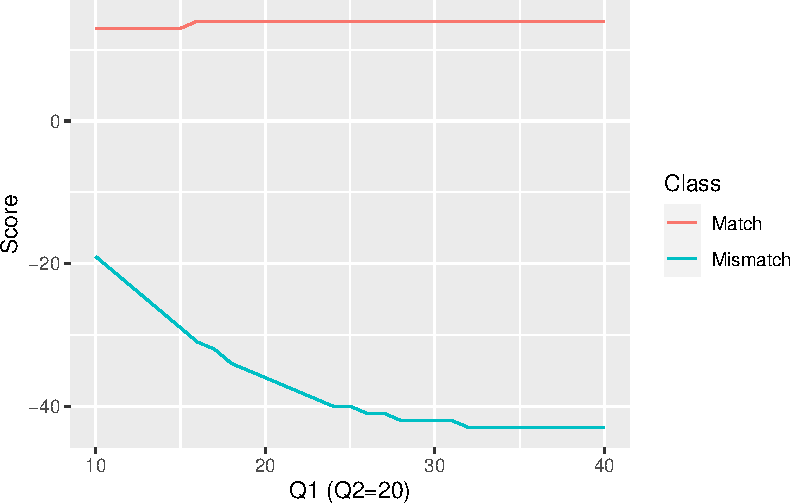
\includegraphics{./comm_computation_files/figure-pdf/unnamed-chunk-1-1.pdf}

}

\caption{Evolution of the match and mismatch scores when the quality of
base is 20 while the second range from 10 to 40.}

\end{figure}

\hypertarget{obimultiplex}{%
\section{\texorpdfstring{\texttt{obimultiplex}}{obimultiplex}}\label{obimultiplex}}

\begin{quote}
Replace the \texttt{ngsfilter} original \emph{OBITools}
\end{quote}

\hypertarget{obicomplement}{%
\section{\texorpdfstring{\texttt{obicomplement}}{obicomplement}}\label{obicomplement}}

\hypertarget{obiclean}{%
\section{\texorpdfstring{\texttt{obiclean}}{obiclean}}\label{obiclean}}

\hypertarget{obiuniq}{%
\section{\texorpdfstring{\texttt{obiuniq}}{obiuniq}}\label{obiuniq}}

\hypertarget{sequence-sampling-and-filtering}{%
\chapter{Sequence sampling and
filtering}\label{sequence-sampling-and-filtering}}

\hypertarget{obigrep-filters-sequence-files-according-to-numerous-conditions}{%
\section{\texorpdfstring{\texttt{obigrep} -- filters sequence files
according to numerous
conditions}{obigrep -- filters sequence files according to numerous conditions}}\label{obigrep-filters-sequence-files-according-to-numerous-conditions}}

The \texttt{obigrep} command is somewhat analogous to the standard Unix
\texttt{grep} command. It selects a subset of sequence records from a
sequence file. A sequence record is a complex object consisting of an
identifier, a set of attributes (a key, defined by its name, associated
with a value), a definition, and the sequence itself. Instead of working
text line by text line like the standard Unix tool, \texttt{obigrep}
selection is done sequence record by sequence record. A large number of
options allow you to refine the selection on any element of the
sequence. \texttt{obigrep} allows you to specify multiple conditions
simultaneously (which take on the value \texttt{TRUE} or \texttt{FALSE})
and only those sequence records which meet all conditions (all
conditions are \texttt{TRUE}) are selected. \texttt{obigrep} is able to
work on two paired read files. The selection criteria apply to one or
the other of the readings in each pair depending on the mode chosen
(\textbf{-\/-paired-mode} option). In all cases the selection is applied
in the same way to both files, thus maintaining their consistency.

\hypertarget{the-options-usable-with-obigrep}{%
\subsection{\texorpdfstring{The options usable with
\texttt{obigrep}}{The options usable with obigrep}}\label{the-options-usable-with-obigrep}}

\hypertarget{selecting-sequences-based-on-their-caracteristics}{%
\subsubsection{Selecting sequences based on their
caracteristics}\label{selecting-sequences-based-on-their-caracteristics}}

Sequences can be selected on several of their caracteristics, their
length, their id, their sequence. Options allow for specifying the
condition if selection.

\begin{description}
\item[\textbf{-\/-min-count} \textbar{} \textbf{-c} \emph{COUNT}]
only sequences reprensenting at least \emph{COUNT} reads will be
selected. That option rely on the \texttt{count} attribute. If the
\texttt{count} attribute is not defined for a sequence record, it is
assumed equal to \(1\).
\item[\textbf{-\/-max-count} \textbar{} \textbf{-C} \emph{COUNT}]
only sequences reprensenting no more than \emph{COUNT} reads will be
selected. That option rely on the \texttt{count} attribute. If the
\texttt{count} attribute is not defined for a sequence record, it is
assumed equal to \(1\).
\item[Example]
Selecting sequence records representing at least five reads in the
dataset.
\end{description}

\begin{Shaded}
\begin{Highlighting}[]
\ExtensionTok{obigrep} \AttributeTok{{-}c}\NormalTok{ 5 data\_SPER01.fasta }\OperatorTok{\textgreater{}}\NormalTok{ data\_norare\_SPER01.fasta}
\end{Highlighting}
\end{Shaded}

\hypertarget{utilities}{%
\chapter{Utilities}\label{utilities}}

\hypertarget{obicount}{%
\section{\texorpdfstring{\texttt{obicount}}{obicount}}\label{obicount}}

\texttt{obicount} counts the number of sequence records, the sum of the
\texttt{count} attributes, and the sum of the length of all the
sequences.

\emph{Example:}

\begin{Shaded}
\begin{Highlighting}[]
\ExtensionTok{obicount}\NormalTok{ seq.fasta  }
\end{Highlighting}
\end{Shaded}

Prints the number of sequence records contained in the
\texttt{seq.fasta} file and the sum of their \texttt{count} attributes.

\emph{Options specific to the command}

\begin{itemize}
\tightlist
\item
  \texttt{-\/-reads\textbar{}-r} Prints read counts.
\item
  \texttt{-\/-symbols\textbar{}-s} Prints symbol counts.
\item
  \texttt{-\/-variants\textbar{}-v} Prints variant counts.
\end{itemize}

\hypertarget{obidistribute}{%
\section{\texorpdfstring{\texttt{obidistribute}}{obidistribute}}\label{obidistribute}}

\hypertarget{obifind}{%
\section{\texorpdfstring{\texttt{obifind}}{obifind}}\label{obifind}}

\begin{quote}
Replace the \texttt{ecofind} original \emph{OBITools.}
\end{quote}

\part{The GO \emph{OBITools} library}

\hypertarget{biosequence}{%
\section*{BioSequence}\label{biosequence}}
\addcontentsline{toc}{section}{BioSequence}

\markright{BioSequence}

The \texttt{BioSequence} class is used to represent biological
sequences. It allows for storing : - the sequence itself as a
\texttt{{[}{]}byte} - the sequencing quality score as a
\texttt{{[}{]}byte} if needed - an identifier as a \texttt{string} - a
definition as a \texttt{string} - a set of \emph{(key, value)} pairs in
a \texttt{map{[}sting{]}interface\{\}}

BioSequence is defined in the obiseq module and is included using the
code

\begin{Shaded}
\begin{Highlighting}[]
\KeywordTok{import} \OperatorTok{(}
    \StringTok{"git.metabarcoding.org/lecasofts/go/obitools/pkg/obiseq"}
\OperatorTok{)}
\end{Highlighting}
\end{Shaded}

\hypertarget{creating-new-instances}{%
\subsection*{Creating new instances}\label{creating-new-instances}}
\addcontentsline{toc}{subsection}{Creating new instances}

To create new instance, use

\begin{itemize}
\tightlist
\item
  \texttt{MakeBioSequence(id\ string,\ sequence\ {[}{]}byte,\ definition\ string)\ obiseq.BioSequence}
\item
  \texttt{NewBioSequence(id\ string,\ sequence\ {[}{]}byte,\ definition\ string)\ *obiseq.BioSequence}
\end{itemize}

Both create a \texttt{BioSequence} instance, but when the first one
returns the instance, the second returns a pointer on the new instance.
Two other functions \texttt{MakeEmptyBioSequence}, and
\texttt{NewEmptyBioSequence} do the same job but provide an
uninitialized objects.

\begin{itemize}
\tightlist
\item
  \texttt{id} parameters corresponds to the unique identifier of the
  sequence. It mist be a string constituted of a single word (not
  containing any space).
\item
  \texttt{sequence} is the DNA sequence itself, provided as a
  \texttt{byte} array (\texttt{{[}{]}byte}).
\item
  \texttt{definition} is a \texttt{string}, potentially empty, but
  usualy containing a sentence explaining what is that sequence.
\end{itemize}

\begin{Shaded}
\begin{Highlighting}[]
\KeywordTok{import} \OperatorTok{(}
    \StringTok{"git.metabarcoding.org/lecasofts/go/obitools/pkg/obiseq"}
\OperatorTok{)}

\KeywordTok{func}\NormalTok{ main}\OperatorTok{()} \OperatorTok{\{}
\NormalTok{    myseq }\OperatorTok{:=}\NormalTok{ obiseq}\OperatorTok{.}\NormalTok{NewBiosequence}\OperatorTok{(}
        \StringTok{"seq\_GH0001"}\OperatorTok{,}
\NormalTok{        bytes}\OperatorTok{.}\NormalTok{FromString}\OperatorTok{(}\StringTok{"ACGTGTCAGTCG"}\OperatorTok{),}
        \StringTok{"A short test sequence"}\OperatorTok{,}
        \OperatorTok{)}
\OperatorTok{\}}
\end{Highlighting}
\end{Shaded}

When formated as fasta the parameters correspond to the following schema

\begin{verbatim}
>id definition containing potentially several words
sequence
\end{verbatim}

\hypertarget{end-of-life-of-a-biosequence-instance}{%
\subsection*{\texorpdfstring{End of life of a \texttt{BioSequence}
instance}{End of life of a BioSequence instance}}\label{end-of-life-of-a-biosequence-instance}}
\addcontentsline{toc}{subsection}{End of life of a \texttt{BioSequence}
instance}

When an instance of \texttt{BioSequence} is no longer in use, it is
normally taken over by the GO garbage collector. If you know that an
instance will never be used again, you can, if you wish, call the
\texttt{Recycle} method on it to store the allocated memory elements in
a \texttt{pool} to limit the allocation effort when many sequences are
being handled. Once the recycle method has been called on an instance,
you must ensure that no other method is called on it.

\hypertarget{accessing-to-the-elements-of-a-sequence}{%
\subsection*{Accessing to the elements of a
sequence}\label{accessing-to-the-elements-of-a-sequence}}
\addcontentsline{toc}{subsection}{Accessing to the elements of a
sequence}

The different elements of an \texttt{obiseq.BioSequence} must be
accessed using a set of methods. For the three main elements provided
during the creation of a new instance methodes are :

\begin{itemize}
\tightlist
\item
  \texttt{Id()\ string}
\item
  \texttt{Sequence()\ {[}{]}byte}
\item
  \texttt{Definition()\ string}
\end{itemize}

It exists pending method to change the value of these elements

\begin{itemize}
\tightlist
\item
  \texttt{SetId(id\ string)}
\item
  \texttt{SetSequence(sequence\ {[}{]}byte)}
\item
  \texttt{SetDefinition(definition\ string)}
\end{itemize}

\begin{Shaded}
\begin{Highlighting}[]
\KeywordTok{import} \OperatorTok{(}
    \StringTok{"fmt"}
    \StringTok{"git.metabarcoding.org/lecasofts/go/obitools/pkg/obiseq"}
\OperatorTok{)}

\KeywordTok{func}\NormalTok{ main}\OperatorTok{()} \OperatorTok{\{}
\NormalTok{    myseq }\OperatorTok{:=}\NormalTok{ obiseq}\OperatorTok{.}\NormalTok{NewBiosequence}\OperatorTok{(}
        \StringTok{"seq\_GH0001"}\OperatorTok{,}
\NormalTok{        bytes}\OperatorTok{.}\NormalTok{FromString}\OperatorTok{(}\StringTok{"ACGTGTCAGTCG"}\OperatorTok{),}
        \StringTok{"A short test sequence"}\OperatorTok{,}
        \OperatorTok{)}

\NormalTok{    fmt}\OperatorTok{.}\NormalTok{Println}\OperatorTok{(}\NormalTok{myseq}\OperatorTok{.}\NormalTok{Id}\OperatorTok{())}
\NormalTok{    myseq}\OperatorTok{.}\NormalTok{SetId}\OperatorTok{(}\StringTok{"SPE01\_0001"}\OperatorTok{)}
\NormalTok{    fmt}\OperatorTok{.}\NormalTok{Println}\OperatorTok{(}\NormalTok{myseq}\OperatorTok{.}\NormalTok{Id}\OperatorTok{())}
\OperatorTok{\}}
\end{Highlighting}
\end{Shaded}

\hypertarget{different-ways-for-accessing-an-editing-the-sequence}{%
\subsubsection*{Different ways for accessing an editing the
sequence}\label{different-ways-for-accessing-an-editing-the-sequence}}
\addcontentsline{toc}{subsubsection}{Different ways for accessing an
editing the sequence}

If \texttt{Sequence()}and \texttt{SetSequence(sequence\ {[}{]}byte)}
methods are the basic ones, several other methods exist.

\begin{itemize}
\tightlist
\item
  \texttt{String()\ string} return the sequence directly converted to a
  \texttt{string} instance.
\item
  The \texttt{Write} method family allows for extending an existing
  sequence following the buffer protocol.

  \begin{itemize}
  \tightlist
  \item
    \texttt{Write(data\ {[}{]}byte)\ (int,\ error)} allows for appending
    a byte array on 3' end of the sequence.
  \item
    \texttt{WriteString(data\ string)\ (int,\ error)} allows for
    appending a \texttt{string}.
  \item
    \texttt{WriteByte(data\ byte)\ error} allows for appending a single
    \texttt{byte}.
  \end{itemize}
\end{itemize}

The \texttt{Clear} method empties the sequence buffer.

\begin{Shaded}
\begin{Highlighting}[]
\KeywordTok{import} \OperatorTok{(}
    \StringTok{"fmt"}
    \StringTok{"git.metabarcoding.org/lecasofts/go/obitools/pkg/obiseq"}
\OperatorTok{)}

\KeywordTok{func}\NormalTok{ main}\OperatorTok{()} \OperatorTok{\{}
\NormalTok{    myseq }\OperatorTok{:=}\NormalTok{ obiseq}\OperatorTok{.}\NormalTok{NewEmptyBiosequence}\OperatorTok{()}

\NormalTok{    myseq}\OperatorTok{.}\NormalTok{WriteString}\OperatorTok{(}\StringTok{"accc"}\OperatorTok{)}
\NormalTok{    myseq}\OperatorTok{.}\NormalTok{WriteByte}\OperatorTok{(}\DataTypeTok{byte}\OperatorTok{(}\CharTok{\textquotesingle{}c\textquotesingle{}}\OperatorTok{))}
\NormalTok{    fmt}\OperatorTok{.}\NormalTok{Println}\OperatorTok{(}\NormalTok{myseq}\OperatorTok{.}\NormalTok{String}\OperatorTok{())}
\OperatorTok{\}}
\end{Highlighting}
\end{Shaded}

\hypertarget{sequence-quality-scores-1}{%
\subsubsection*{Sequence quality
scores}\label{sequence-quality-scores-1}}
\addcontentsline{toc}{subsubsection}{Sequence quality scores}

Sequence quality scores cannot be initialized at the time of instance
creation. You must use dedicated methods to add quality scores to a
sequence.

To be coherent the length of both the DNA sequence and que quality score
sequence must be equal. But assessment of this constraint is realized.
It is of the programmer responsability to check that invariant.

While accessing to the quality scores relies on the method
\texttt{Quality()\ {[}{]}byte}, setting the quality need to call one of
the following method. They run similarly to their sequence dedicated
conterpart.

\begin{itemize}
\tightlist
\item
  \texttt{SetQualities(qualities\ Quality)}
\item
  \texttt{WriteQualities(data\ {[}{]}byte)\ (int,\ error)}
\item
  \texttt{WriteByteQualities(data\ byte)\ error}
\end{itemize}

In a way analogous to the \texttt{Clear} method,
\texttt{ClearQualities()} empties the sequence of quality scores.

\hypertarget{the-annotations-of-a-sequence}{%
\subsection*{The annotations of a
sequence}\label{the-annotations-of-a-sequence}}
\addcontentsline{toc}{subsection}{The annotations of a sequence}

A sequence can be annotated with attributes. Each attribute is
associated with a value. An attribute is identified by its name. The
name of an attribute consists of a character string containing no spaces
or blank characters. Values can be of several types.

\begin{itemize}
\tightlist
\item
  Scalar types:

  \begin{itemize}
  \tightlist
  \item
    integer
  \item
    numeric
  \item
    character
  \item
    boolean
  \end{itemize}
\item
  Container types:

  \begin{itemize}
  \tightlist
  \item
    vector
  \item
    map
  \end{itemize}
\end{itemize}

Vectors can contain any type of scalar. Maps are compulsorily indexed by
strings and can contain any scalar type. It is not possible to have
nested container type.

Annotations are stored in an object of type \texttt{bioseq.Annotation}
which is an alias of \texttt{map{[}string{]}interface\{\}}. This map can
be retrieved using the \texttt{Annotations()\ Annotation} method. If no
annotation has been defined for this sequence, the method returns an
empty map. It is possible to test an instance of \texttt{BioSequence}
using its \texttt{HasAnnotation()\ bool} method to see if it has any
annotations associated with it.

\begin{itemize}
\tightlist
\item
  GetAttribute(key string) (interface\{\}, bool)
\end{itemize}

\hypertarget{the-sequence-iterator}{%
\section*{The sequence iterator}\label{the-sequence-iterator}}
\addcontentsline{toc}{section}{The sequence iterator}

\markright{The sequence iterator}

The pakage \emph{obiter} provides an iterator mecanism for manipulating
sequences. The main class provided by this package is
\texttt{obiiter.IBioSequence}. An \texttt{IBioSequence} iterator
provides batch of sequences.

\hypertarget{basic-usage-of-a-sequence-iterator}{%
\subsection*{Basic usage of a sequence
iterator}\label{basic-usage-of-a-sequence-iterator}}
\addcontentsline{toc}{subsection}{Basic usage of a sequence iterator}

Many functions, among them functions reading sequences from a text file,
return a \texttt{IBioSequence} iterator. The iterator class provides two
main methods:

\begin{itemize}
\tightlist
\item
  \texttt{Next()\ bool}
\item
  \texttt{Get()\ obiiter.BioSequenceBatch}
\end{itemize}

The \texttt{Next} method moves the iterator to the next value, while the
\texttt{Get} method returns the currently pointed value. Using them, it
is possible to loop over the data as in the following code chunk.

\begin{Shaded}
\begin{Highlighting}[]
\KeywordTok{import} \OperatorTok{(}
    \StringTok{"git.metabarcoding.org/lecasofts/go/obitools/pkg/obiformats"}
\OperatorTok{)}

\KeywordTok{func}\NormalTok{ main}\OperatorTok{()} \OperatorTok{\{}
\NormalTok{    mydata }\OperatorTok{:=}\NormalTok{ obiformats}\OperatorTok{.}\NormalTok{ReadFastSeqFromFile}\OperatorTok{(}\StringTok{"myfile.fasta"}\OperatorTok{)}
       
    \ControlFlowTok{for}\NormalTok{ mydata}\OperatorTok{.}\NormalTok{Next}\OperatorTok{()} \OperatorTok{\{}
\NormalTok{        data }\OperatorTok{:=}\NormalTok{ mydata}\OperatorTok{.}\NormalTok{Get}\OperatorTok{()}
        \CommentTok{//}
        \CommentTok{// Whatever you want to do with the data chunk}
        \CommentTok{//}
    \OperatorTok{\}}
\OperatorTok{\}}
\end{Highlighting}
\end{Shaded}

An \texttt{obiseq.BioSequenceBatch} instance is a set of sequences
stored in an \texttt{obiseq.BioSequenceSlice} and a sequence number. The
number of sequences in a batch is not defined. A batch can even contain
zero sequences, if for example all sequences initially included in the
batch have been filtered out at some stage of their processing.

\hypertarget{the-pipable-functions}{%
\subsection*{\texorpdfstring{The \texttt{Pipable}
functions}{The Pipable functions}}\label{the-pipable-functions}}
\addcontentsline{toc}{subsection}{The \texttt{Pipable} functions}

A function consuming a \texttt{obiiter.IBioSequence} and returning a
\texttt{obiiter.IBioSequence} is of class \texttt{obiiter.Pipable}.

\hypertarget{the-teeable-functions}{%
\subsection*{\texorpdfstring{The \texttt{Teeable}
functions}{The Teeable functions}}\label{the-teeable-functions}}
\addcontentsline{toc}{subsection}{The \texttt{Teeable} functions}

A function consuming a \texttt{obiiter.IBioSequence} and returning two
\texttt{obiiter.IBioSequence} instance is of class
\texttt{obiiter.Teeable}.

\appendix
\addcontentsline{toc}{part}{Appendices}

\hypertarget{annexes}{%
\chapter{Annexes}\label{annexes}}

\hypertarget{sequence-attributes}{%
\subsection{Sequence attributes}\label{sequence-attributes}}

\hypertarget{reserved-sequence-attributes}{%
\subsubsection{Reserved sequence
attributes}\label{reserved-sequence-attributes}}

\hypertarget{ali_dir}{%
\paragraph{\texorpdfstring{\texttt{ali\_dir}}{ali\_dir}}\label{ali_dir}}

\hypertarget{type-string}{%
\subparagraph{\texorpdfstring{Type :
\texttt{string}}{Type : string}}\label{type-string}}

The attribute can contain 2 string values \texttt{"left"} or
\texttt{"right".}

\hypertarget{set-by-the-obipairing-tool}{%
\subparagraph{\texorpdfstring{Set by the \emph{obipairing}
tool}{Set by the obipairing tool}}\label{set-by-the-obipairing-tool}}

The alignment generated by \emph{obipairing} is a 3'-end gap free
algorithm. Two cases can occur when aligning the forward and reverse
reads. If the barcode is long enough, both the reads overlap only on
their 3' ends. In such case, the alignment direction \texttt{ali\_dir}
is set to \emph{left}. If the barcode is shorter than the read length,
the paired reads overlap by their 5' ends, and the complete barcode is
sequenced by both the reads. In that later case, \texttt{ali\_dir} is
set to \emph{right}.

\hypertarget{ali_length}{%
\paragraph{\texorpdfstring{\texttt{ali\_length}}{ali\_length}}\label{ali_length}}

\hypertarget{set-by-the-obipairing-tool-1}{%
\subparagraph{\texorpdfstring{Set by the \emph{obipairing}
tool}{Set by the obipairing tool}}\label{set-by-the-obipairing-tool-1}}

Length of the aligned parts when merging forward and reverse reads

\hypertarget{count-the-number-of-sequence-occurrences}{%
\paragraph{\texorpdfstring{\texttt{count} : the number of sequence
occurrences}{count : the number of sequence occurrences}}\label{count-the-number-of-sequence-occurrences}}

\hypertarget{set-by-the-obiuniq-tool}{%
\subparagraph{\texorpdfstring{Set by the \emph{obiuniq}
tool}{Set by the obiuniq tool}}\label{set-by-the-obiuniq-tool}}

The \texttt{count} attribute indicates how-many strictly identical
sequences have been merged in a single record. It contains an integer
value. If it is absent this means that the sequence record represents a
single occurrence of the sequence.

\hypertarget{getter-method-count}{%
\subparagraph{\texorpdfstring{Getter : method
\texttt{Count()}}{Getter : method Count()}}\label{getter-method-count}}

The \texttt{Count()} method allows to access to the count attribute as
an integer value. If the \texttt{count} attribute is not defined for the
given sequence, the value \emph{1} is returned

\hypertarget{merged_}{%
\paragraph{\texorpdfstring{\texttt{merged\_*}}{merged\_*}}\label{merged_}}

\hypertarget{type-mapstringint}{%
\subparagraph{\texorpdfstring{Type :
\texttt{map{[}string{]}int}}{Type : map{[}string{]}int}}\label{type-mapstringint}}

\hypertarget{set-by-the-obiuniq-tool-1}{%
\subparagraph{\texorpdfstring{Set by the \emph{obiuniq}
tool}{Set by the obiuniq tool}}\label{set-by-the-obiuniq-tool-1}}

The \texttt{-m} option of the \emph{obiuniq} tools allows for keeping
track of the distribution of the values stored in given attribute of
interest. Often this option is used to summarise distribution of a
sequence variant accross samples when \emph{obiuniq} is run after
running \emph{obimultiplex}. The actual name of the attribute depends on
the name of the monitored attribute. If \texttt{-m} option is used with
the attribute \emph{sample}, then this attribute names
\emph{merged\_sample}.

\hypertarget{mode}{%
\paragraph{\texorpdfstring{\texttt{mode}}{mode}}\label{mode}}

\hypertarget{set-by-the-obipairing-tool-2}{%
\subparagraph{\texorpdfstring{Set by the \emph{obipairing}
tool}{Set by the obipairing tool}}\label{set-by-the-obipairing-tool-2}}

\textbf{\texttt{obitag\_ref\_index}}

\hypertarget{set-by-the-obirefidx-tool.}{%
\subparagraph{\texorpdfstring{Set by the \emph{obirefidx}
tool.}{Set by the obirefidx tool.}}\label{set-by-the-obirefidx-tool.}}

It resumes to which taxonomic annotation a match to that sequence must
lead according to the number of differences existing between the query
sequence and the reference sequence having that tag.

\hypertarget{getter-method-count-1}{%
\subparagraph{\texorpdfstring{Getter : method
\texttt{Count()}}{Getter : method Count()}}\label{getter-method-count-1}}

\hypertarget{pairing_mismatches}{%
\paragraph{\texorpdfstring{\texttt{pairing\_mismatches}}{pairing\_mismatches}}\label{pairing_mismatches}}

\hypertarget{set-by-the-obipairing-tool-3}{%
\subparagraph{\texorpdfstring{Set by the \emph{obipairing}
tool}{Set by the obipairing tool}}\label{set-by-the-obipairing-tool-3}}

\hypertarget{score}{%
\paragraph{\texorpdfstring{\texttt{score}}{score}}\label{score}}

\hypertarget{set-by-the-obipairing-tool-4}{%
\subparagraph{\texorpdfstring{Set by the \emph{obipairing}
tool}{Set by the obipairing tool}}\label{set-by-the-obipairing-tool-4}}

\hypertarget{score_norm}{%
\paragraph{\texorpdfstring{\texttt{score\_norm}}{score\_norm}}\label{score_norm}}

\hypertarget{set-by-the-obipairing-tool-5}{%
\subparagraph{\texorpdfstring{Set by the \emph{obipairing}
tool}{Set by the obipairing tool}}\label{set-by-the-obipairing-tool-5}}

\hypertarget{references}{%
\chapter*{References}\label{references}}
\addcontentsline{toc}{chapter}{References}

\markboth{References}{References}

\hypertarget{refs}{}
\begin{CSLReferences}{1}{0}
\leavevmode\vadjust pre{\hypertarget{ref-Andersen2012-gj}{}}%
Andersen, Kenneth, Karen Lise Bird, Morten Rasmussen, James Haile,
Henrik Breuning-Madsen, Kurt H Kjaer, Ludovic Orlando, M Thomas P
Gilbert, and Eske Willerslev. 2012. {``{Meta-barcoding of {ë}dirt{ı́}DNA
from soil reflects vertebrate biodiversity}.''} \emph{Molecular Ecology}
21 (8): 1966--79.

\leavevmode\vadjust pre{\hypertarget{ref-Baldwin2013-yc}{}}%
Baldwin, Darren S, Matthew J Colloff, Gavin N Rees, Anthony A Chariton,
Garth O Watson, Leon N Court, Diana M Hartley, et al. 2013. {``{Impacts
of inundation and drought on eukaryote biodiversity in semi-arid
floodplain soils}.''} \emph{Molecular Ecology} 22 (6): 1746--58.
\url{https://doi.org/10.1111/mec.12190}.

\leavevmode\vadjust pre{\hypertarget{ref-Boyer2016-gq}{}}%
Boyer, Frédéric, Céline Mercier, Aurélie Bonin, Yvan Le Bras, Pierre
Taberlet, and Eric Coissac. 2016. {``{obitools: a unix-inspired software
package for DNA metabarcoding}.''} \emph{Molecular Ecology Resources} 16
(1): 176--82. \url{https://doi.org/10.1111/1755-0998.12428}.

\leavevmode\vadjust pre{\hypertarget{ref-Caporaso2010-ii}{}}%
Caporaso, J Gregory, Justin Kuczynski, Jesse Stombaugh, Kyle Bittinger,
Frederic D Bushman, Elizabeth K Costello, Noah Fierer, et al. 2010.
{``{QIIME allows analysis of high-throughput community sequencing
data}.''} \emph{Nature Methods} 7 (5): 335--36.
\url{https://doi.org/10.1038/nmeth.f.303}.

\leavevmode\vadjust pre{\hypertarget{ref-Chariton2010-cz}{}}%
Chariton, Anthony A, Anthony C Roach, Stuart L Simpson, and Graeme E
Batley. 2010. {``{Influence of the choice of physical and chemistry
variables on interpreting patterns of sediment contaminants and their
relationships with estuarine macrobenthic communities}.''} \emph{Marine
and Freshwater Research}. \url{https://doi.org/10.1071/mf09263}.

\leavevmode\vadjust pre{\hypertarget{ref-cock2010sanger}{}}%
Cock, Peter JA, Christopher J Fields, Naohisa Goto, Michael L Heuer, and
Peter M Rice. 2010. {``The Sanger FASTQ File Format for Sequences with
Quality Scores, and the Solexa/Illumina FASTQ Variants.''} \emph{Nucleic
Acids Research} 38 (6): 1767--71.

\leavevmode\vadjust pre{\hypertarget{ref-Deagle2009-yh}{}}%
Deagle, Bruce E, Roger Kirkwood, and Simon N Jarman. 2009. {``{Analysis
of Australian fur seal diet by pyrosequencing prey DNA in faeces}.''}
\emph{Molecular Ecology} 18 (9): 2022--38.
\url{https://doi.org/10.1111/j.1365-294X.2009.04158.x}.

\leavevmode\vadjust pre{\hypertarget{ref-Kowalczyk2011-kg}{}}%
Kowalczyk, Rafał, Pierre Taberlet, Eric Coissac, Alice Valentini,
Christian Miquel, Tomasz Kamiński, and Jan M Wójcik. 2011. {``{Influence
of management practices on large herbivore diet---Case of European bison
in Bia{ł}owie{ż}a Primeval Forest (Poland)}.''} \emph{Forest Ecology and
Management} 261 (4): 821--28.
\url{https://doi.org/10.1016/j.foreco.2010.11.026}.

\leavevmode\vadjust pre{\hypertarget{ref-Lipman1985-hw}{}}%
Lipman, D J, and W R Pearson. 1985. {``{Rapid and sensitive protein
similarity searches}.''} \emph{Science} 227 (4693): 1435--41.
\url{http://www.ncbi.nlm.nih.gov/pubmed/2983426}.

\leavevmode\vadjust pre{\hypertarget{ref-Parducci2012-rn}{}}%
Parducci, Laura, Tina Jørgensen, Mari Mette Tollefsrud, Ellen Elverland,
Torbjørn Alm, Sonia L Fontana, K D Bennett, et al. 2012. {``{Glacial
survival of boreal trees in northern Scandinavia}.''} \emph{Science} 335
(6072): 1083--86. \url{https://doi.org/10.1126/science.1216043}.

\leavevmode\vadjust pre{\hypertarget{ref-Riaz2011-gn}{}}%
Riaz, Tiayyba, Wasim Shehzad, Alain Viari, François Pompanon, Pierre
Taberlet, and Eric Coissac. 2011. {``{ecoPrimers: inference of new DNA
barcode markers from whole genome sequence analysis}.''} \emph{Nucleic
Acids Research} 39 (21): e145. \url{https://doi.org/10.1093/nar/gkr732}.

\leavevmode\vadjust pre{\hypertarget{ref-Schloss2009-qy}{}}%
Schloss, Patrick D, Sarah L Westcott, Thomas Ryabin, Justine R Hall,
Martin Hartmann, Emily B Hollister, Ryan A Lesniewski, et al. 2009.
{``{Introducing mothur: open-source, platform-independent,
community-supported software for describing and comparing microbial
communities}.''} \emph{Applied and Environmental Microbiology} 75 (23):
7537--41. \url{https://doi.org/10.1128/AEM.01541-09}.

\leavevmode\vadjust pre{\hypertarget{ref-Seguritan2001-tg}{}}%
Seguritan, V, and F Rohwer. 2001. {``{FastGroup: a program to
dereplicate libraries of 16S rDNA sequences}.''} \emph{BMC
Bioinformatics} 2 (October): 9.
\url{https://doi.org/10.1186/1471-2105-2-9}.

\leavevmode\vadjust pre{\hypertarget{ref-Shehzad2012-pn}{}}%
Shehzad, Wasim, Tiayyba Riaz, Muhammad A Nawaz, Christian Miquel, Carole
Poillot, Safdar A Shah, Francois Pompanon, Eric Coissac, and Pierre
Taberlet. 2012. {``{Carnivore diet analysis based on next-generation
sequencing: Application to the leopard cat (Prionailurus bengalensis) in
Pakistan}.''} \emph{Molecular Ecology} 21 (8): 1951--65.
\url{https://onlinelibrary.wiley.com/doi/abs/10.1111/j.1365-294X.2011.05424.x}.

\leavevmode\vadjust pre{\hypertarget{ref-Sogin2006-ab}{}}%
Sogin, Mitchell L, Hilary G Morrison, Julie A Huber, David Mark Welch,
Susan M Huse, Phillip R Neal, Jesus M Arrieta, and Gerhard J Herndl.
2006. {``{Microbial diversity in the deep sea and the underexplored
"rare biosphere"}.''} \emph{Proceedings of the National Academy of
Sciences of the United States of America} 103 (32): 12115--20.
\url{https://doi.org/10.1073/pnas.0605127103}.

\leavevmode\vadjust pre{\hypertarget{ref-Sonstebo2010-vv}{}}%
Sønstebø, J H, L Gielly, A K Brysting, R Elven, M Edwards, J Haile, E
Willerslev, et al. 2010. {``{Using next-generation sequencing for
molecular reconstruction of past Arctic vegetation and climate}.''}
\emph{Molecular Ecology Resources} 10 (6): 1009--18.
\url{https://doi.org/10.1111/j.1755-0998.2010.02855.x}.

\leavevmode\vadjust pre{\hypertarget{ref-Taberlet2012-pf}{}}%
Taberlet, Pierre, Eric Coissac, Mehrdad Hajibabaei, and Loren H
Rieseberg. 2012. {``{Environmental DNA}.''} \emph{Molecular Ecology} 21
(8): 1789--93. \url{https://doi.org/10.1111/j.1365-294X.2012.05542.x}.

\leavevmode\vadjust pre{\hypertarget{ref-Thomsen2012-au}{}}%
Thomsen, Philip Francis, Jos Kielgast, Lars L Iversen, Carsten Wiuf,
Morten Rasmussen, M Thomas P Gilbert, Ludovic Orlando, and Eske
Willerslev. 2012. {``{Monitoring endangered freshwater biodiversity
using environmental DNA}.''} \emph{Molecular Ecology} 21 (11): 2565--73.
\url{https://doi.org/10.1111/j.1365-294X.2011.05418.x}.

\leavevmode\vadjust pre{\hypertarget{ref-Valentini2009-ay}{}}%
Valentini, Alice, Christian Miquel, Muhammad Ali Nawaz, Eva Bellemain,
Eric Coissac, François Pompanon, Ludovic Gielly, et al. 2009. {``{New
perspectives in diet analysis based on DNA barcoding and parallel
pyrosequencing: the trnL approach}.''} \emph{Molecular Ecology
Resources} 9 (1): 51--60.
\url{https://doi.org/10.1111/j.1755-0998.2008.02352.x}.

\leavevmode\vadjust pre{\hypertarget{ref-Yoccoz2012-ix}{}}%
Yoccoz, N G, K A Bråthen, L Gielly, J Haile, M E Edwards, T Goslar, H
Von Stedingk, et al. 2012. {``{DNA from soil mirrors plant taxonomic and
growth form diversity}.''} \emph{Molecular Ecology} 21 (15): 3647--55.
\url{https://doi.org/10.1111/j.1365-294X.2012.05545.x}.

\end{CSLReferences}



\end{document}
